\chapter{Electrons in a Periodic Potential}

An electron in a crystal moves in a potential with the periodicity of the lattice, and that single fact --- before any approximation whatsoever --- already fixes the form of the stationary states. This chapter begins with Bloch's theorem and its immediate consequences: the labelling of states by a crystal momentum and a band index, the notion of a Fermi surface, and the density of levels. It then treats the two complementary limits in which the problem becomes tractable. In the \emph{nearly free electron} limit the periodic potential is a weak perturbation on plane waves, and its only dramatic effect is to open gaps at the Bragg planes. In the \emph{tight-binding} limit we start instead from atomic orbitals localized on each site and let a small overlap between neighbours broaden the discrete atomic levels into bands. We then collect the lattice Fourier identities that both pictures rest on, and close with the semiclassical dynamics of Bloch wavepackets.

A word on notation. We write the electron position as $\lvect{x}$, reserving $\cvect{R}$ for direct lattice vectors and $\cvect{G}$ for reciprocal lattice vectors, with wavevectors $\lvect{k}$ and $\lvect{q}$.

% ============================================================
\section{Bloch's Theorem}
% ============================================================

Throughout we make two assumptions: that the crystal is perfect, i.e.\ a strictly periodic array of atoms, and that the atomic nuclei are static. The potential is then periodic,
\begin{equation}
    U(\lvect{x}+\cvect{R}) = U(\lvect{x}),
\end{equation}
for every lattice vector $\cvect{R}$, and the one-electron Schrödinger equation
\begin{equation}
    \hat{H}\psi = \left( -\frac{\hbar^2}{2m}\nabla^2 + U(\lvect{x}) \right)\psi = E\psi
\end{equation}
has a Hamiltonian that is periodic in $\lvect{x}$.

\begin{theorem}[Bloch's theorem]
The eigenstates $\psi$ of the one-electron Hamiltonian $H = -\hbar^2\nabla^2/2m + U(\lvect{x})$ with $U$ periodic can be chosen to have the form
\begin{equation}
    \psi_{n\lvect{k}}(\lvect{x}) = e^{i\lvect{k}\cdot\lvect{x}}\, u_{n\lvect{k}}(\lvect{x}),
    \qquad u_{n\lvect{k}}(\lvect{x}+\cvect{R}) = u_{n\lvect{k}}(\lvect{x}),
\end{equation}
equivalently
\begin{equation}
    \psi_{n\lvect{k}}(\lvect{x}+\cvect{R}) = e^{i\lvect{k}\cdot\cvect{R}}\, \psi_{n\lvect{k}}(\lvect{x}).
    \label{eq:bloch-condition}
\end{equation}
\end{theorem}

\subsection{First Proof: Translation Operators}

Define the translation operator $T_{\cvect{R}}$ by $T_{\cvect{R}} f(\lvect{x}) \equiv f(\lvect{x}+\cvect{R})$. Because the Hamiltonian is periodic,
\begin{equation}
    T_{\cvect{R}} \hat{H} \psi = \hat{H}(\lvect{x}+\cvect{R})\psi(\lvect{x}+\cvect{R}) = H(\lvect{x})\psi(\lvect{x}+\cvect{R}) = \hat{H} T_{\cvect{R}}\psi,
\end{equation}
so $T_{\cvect{R}}$ commutes with $H$. The translations also commute among themselves,
\begin{equation}
    T_{\cvect{R}} T_{\cvect{R}'} \psi(\lvect{x}) = \psi(\lvect{x}+\cvect{R}+\cvect{R}') = T_{\cvect{R}'} T_{\cvect{R}} \psi = T_{\cvect{R}+\cvect{R}'}\psi.
\end{equation}
Hence $\{T_{\cvect{R}}\}$ and $H$ form a set of commuting operators and can be simultaneously diagonalized:
\begin{equation}
    \hat{H}\psi = E\psi, \qquad T_{\cvect{R}}\psi = C(\cvect{R})\psi,
\end{equation}
where the multiplicative property $C(\cvect{R}+\cvect{R}') = C(\cvect{R})C(\cvect{R}')$ lets us write the eigenvalues on the primitive vectors as
\begin{equation}
    C(\lvect{a}_i) = \exp(2\pi i x_i).
\end{equation}
For an arbitrary lattice vector $\cvect{R} = n_1\lvect{a}_1 + n_2\lvect{a}_2 + n_3\lvect{a}_3$,
\begin{equation}
    C(\cvect{R}) = C(\lvect{a}_1)^{n_1} C(\lvect{a}_2)^{n_2} C(\lvect{a}_3)^{n_3}
    = \exp\bigl(2\pi i x_1 n_1 + 2\pi i x_2 n_2 + 2\pi i x_3 n_3\bigr).
\end{equation}
Now take $\lvect{k} = x_1\lvect{b}_1 + x_2\lvect{b}_2 + x_3\lvect{b}_3$, where the $\lvect{b}_i$ are the reciprocal primitive vectors satisfying $\lvect{b}_i\cdot\lvect{a}_j = 2\pi\delta_{ij}$. Then
\begin{equation}
    \exp(i\lvect{k}\cdot\cvect{R}) = \exp\bigl(i(x_1\lvect{b}_1 + x_2\lvect{b}_2 + x_3\lvect{b}_3)\cdot(n_1\lvect{a}_1 + n_2\lvect{a}_2 + n_3\lvect{a}_3)\bigr)
    = \exp\bigl(i(2\pi x_1 n_1 + 2\pi x_2 n_2 + 2\pi x_3 n_3)\bigr) = C(\cvect{R}),
\end{equation}
so that $T_{\cvect{R}}\psi = \psi(\lvect{x}+\cvect{R}) = C(\cvect{R})\psi = e^{i\lvect{k}\cdot\cvect{R}}\psi$, which is exactly~\eqref{eq:bloch-condition}.

\subsection{Born--von Karman Boundary Conditions}

\begin{definition}[Born--von Karman boundary condition]
\begin{equation}
    \psi(\lvect{x} + N_i \lvect{a}_i) = \psi(\lvect{x}), \qquad i = 1,2,3,
\end{equation}
where $N = N_1 N_2 N_3$ is the total number of primitive cells and $N_i$ is the length of the system in unit cells along a particular direction.
\end{definition}

This constrains $\lvect{k}$ to be real and quantizes its allowed values. Applying the Bloch condition,
\begin{equation}
    \psi_{n\lvect{k}}(\lvect{x}+N_i\lvect{a}_i) = \exp(iN_i \lvect{k}\cdot\lvect{a}_i)\, \psi_{n\lvect{k}}(\lvect{x}) = \psi(\lvect{x})
    \;\Longrightarrow\; \exp(iN_i\lvect{k}\cdot\lvect{a}_i) = 1
    \;\Longrightarrow\; \lvect{k}\cdot\lvect{a}_i = \frac{2\pi m}{N_i}, \quad m \in \mathbb{Z}.
\end{equation}
Writing $\lvect{k} = x_1\lvect{b}_1 + x_2\lvect{b}_2 + x_3\lvect{b}_3$ gives $2\pi x_i = 2\pi m/N_i$, i.e.\ $x_i = m/N_i$.

\begin{formula}[Allowed wavevectors]
\begin{equation}
    \lvect{k} = \sum_{i=1}^{3} \frac{m_i}{N_i}\,\lvect{b}_i, \qquad m_i \in \mathbb{Z}.
\end{equation}
\end{formula}

\subsection{Volume per Allowed Wavevector}

The allowed $\lvect{k}$ form a lattice whose primitive cell is the parallelepiped with edges $\lvect{b}_i/N_i$, so the volume per $\lvect{k}$-value is
\begin{equation}
    \Delta k = \frac{\lvect{b}_1}{N_1}\cdot\left( \frac{\lvect{b}_2}{N_2} \times \frac{\lvect{b}_3}{N_3} \right)
    = \frac{1}{N}\,\lvect{b}_1\cdot(\lvect{b}_2\times\lvect{b}_3).
\end{equation}

\begin{fact}
The number of allowed wavevectors in a primitive cell of the reciprocal lattice equals the number of sites in the crystal.
\end{fact}

Since the volume of the reciprocal lattice primitive cell is $(2\pi)^3/v$ with $v = V/N$,
\begin{equation}
    \Delta k = \frac{\text{primitive cell volume}}{N} = \frac{(2\pi)^3}{V}.
\end{equation}

\subsection{Second Proof: Fourier Expansion}

The second proof is more laborious but produces the central equation on which the nearly free electron model is built. By Fourier transform, any function obeying the boundary conditions can be written
\begin{equation}
    \psi(\lvect{x}) = \sum_{\lvect{q}} c_{\lvect{q}}\, e^{i\lvect{q}\cdot\lvect{x}},
\end{equation}
where $\lvect{q}$ runs over the set of BVK wavevectors. The potential, being periodic in the lattice, has a plane-wave expansion containing only reciprocal lattice vectors:
\begin{equation}
    U(\lvect{x}) = \sum_{\cvect{G}} U_{\cvect{G}}\, e^{i\cvect{G}\cdot\lvect{x}},
    \qquad
    U_{\cvect{G}} = \frac{1}{v}\int_{\text{cell}} d\lvect{x}\; e^{-i\cvect{G}\cdot\lvect{x}}\, U(\lvect{x}),
\end{equation}
where it suffices to integrate over one cell since $U$ is periodic. We are free to make the constant term vanish,
\begin{equation}
    U_0 = \frac{1}{v}\int_{\text{cell}} d\lvect{x}\; U(\lvect{x}) = 0.
\end{equation}
Since $U(\lvect{x})$ is real, $U_{-\cvect{G}} = U^*_{\cvect{G}}$; and if the lattice has inversion symmetry, $U(\lvect{x}) = U(-\lvect{x})$ for a suitable choice of origin, then $U_{\cvect{G}} = U^*_{-\cvect{G}}$ so that $U_{\cvect{G}}$ is real.

Substituting both expansions into the Schrödinger equation, the kinetic term gives
\begin{equation}
    -\frac{\hbar^2}{2m}\nabla^2 \psi = \sum_{\lvect{q}} \frac{\hbar^2}{2m} q^2 c_{\lvect{q}}\, e^{i\lvect{q}\cdot\lvect{x}},
\end{equation}
while the potential term gives
\begin{equation}
    U\psi = \left( \sum_{\cvect{G}} U_{\cvect{G}} e^{i\cvect{G}\cdot\lvect{x}} \right)\left( \sum_{\lvect{q}} c_{\lvect{q}} e^{i\lvect{q}\cdot\lvect{x}} \right)
    = \sum_{\cvect{G},\lvect{q}} U_{\cvect{G}} c_{\lvect{q}}\, e^{i(\cvect{G}+\lvect{q})\cdot\lvect{x}}
    = \sum_{\cvect{G},\lvect{q}'} U_{\cvect{G}} c_{\lvect{q}'-\cvect{G}}\, e^{i\lvect{q}'\cdot\lvect{x}}.
\end{equation}

\begin{fact}
The potential $U$ only couples a wavevector $\lvect{q}$ to wavevectors differing from it by a reciprocal lattice vector, $\lvect{q}+\cvect{G}$. Everything that follows is a rigorous statement of this fact.
\end{fact}

Collecting terms with a common exponential,
\begin{equation}
    \sum_{\lvect{q}} e^{i\lvect{q}\cdot\lvect{x}} \left\{ \left( \frac{\hbar^2}{2m}q^2 - \varepsilon \right) c_{\lvect{q}} + \sum_{\cvect{G}'} U_{\cvect{G}'}\, c_{\lvect{q}-\cvect{G}'} \right\} = 0,
\end{equation}
and since the plane waves satisfying the Born--von Karman conditions are orthogonal, each brace must vanish separately:
\begin{equation}
    \left( \frac{\hbar^2}{2m}q^2 - \varepsilon \right) c_{\lvect{q}} + \sum_{\cvect{G}'} U_{\cvect{G}'}\, c_{\lvect{q}-\cvect{G}'} = 0
    \qquad \text{for all allowed } \lvect{q}.
\end{equation}
Rewriting with $\lvect{q} = \lvect{k}-\cvect{G}$, so that $\lvect{k}$ lies in the first Brillouin zone, and then shifting $\cvect{G}' \to \cvect{G}'-\cvect{G}$, gives the central equation.

\begin{formula}[Central equation]
\begin{equation}
    \left( \frac{\hbar^2}{2m}(\lvect{k}-\cvect{G})^2 - \varepsilon \right) c_{\lvect{k}-\cvect{G}}
    + \sum_{\cvect{G}'} U_{\cvect{G}'-\cvect{G}}\, c_{\lvect{k}-\cvect{G}'} = 0.
    \label{eq:bloch-central}
\end{equation}
\end{formula}

This relates only the coefficients $c_{\lvect{k}}, c_{\lvect{k}-\cvect{G}}, c_{\lvect{k}-\cvect{G}'}, \ldots$ to one another, so the problem of determining the solution coefficients splits into $N$ independent subproblems, one for each $\lvect{k}$ in the first zone. Organizing the vector of coefficients into reciprocal-space blocks,
\begin{equation}
    \cvect{\Psi} = \bigl( \underbrace{c_{\lvect{k}},\, c_{\lvect{k}-\cvect{G}},\, c_{\lvect{k}-\cvect{G}'},\ldots}_{\lvect{k}},\;
    \underbrace{c_{\lvect{k}'},\, c_{\lvect{k}'-\cvect{G}},\, c_{\lvect{k}'-\cvect{G}'},\ldots}_{\lvect{k}'},\; \ldots \bigr),
\end{equation}
the Hamiltonian is block diagonal, with one block $\hat{H}_{\lvect{k}}$ for each of the $N$ wavevectors.

\begin{formula}[Reduced matrix equation]
\begin{equation}
    \sum_{\cvect{G}'} H_{\cvect{G}\cvect{G}'}(\lvect{k})\, c^n_{\cvect{G}'} = E_n(\lvect{k})\, c^n_{\cvect{G}},
    \qquad
    H_{\cvect{G}\cvect{G}'}(\lvect{k}) \equiv \frac{\hbar^2}{2m}|\lvect{k}+\cvect{G}|^2 \delta_{\cvect{G}\cvect{G}'} + U_{\cvect{G}-\cvect{G}'}.
\end{equation}
\end{formula}

There are thus $N$ independent subproblems of the form $\hat{H}_{\lvect{k}}\psi_{\lvect{k}} = E\psi_{\lvect{k}}$, and the solution for a given $\lvect{k}$ is
\begin{equation}
    \psi_{\lvect{k}}(\lvect{x}) = \sum_{\cvect{G}} c^n_{\cvect{G}}\, e^{i(\lvect{k}+\cvect{G})\cdot\lvect{x}}
    = e^{i\lvect{k}\cdot\lvect{x}} \underbrace{\sum_{\cvect{G}} c^n_{\cvect{G}}\, e^{i\cvect{G}\cdot\lvect{x}}}_{u_{\lvect{k}}(\lvect{x})}.
\end{equation}
Since $u^n_{\lvect{k}}(\lvect{x}+\cvect{R}) = \sum_{\cvect{G}} c^n_{\cvect{G}} e^{i\cvect{G}\cdot(\lvect{x}+\cvect{R})} = \sum_{\cvect{G}} c^n_{\cvect{G}} e^{i\cvect{G}\cdot\lvect{x}} = u^n_{\lvect{k}}(\lvect{x})$, this proves Bloch's theorem a second time.

% ============================================================
\section{Consequences of Bloch's Theorem}
% ============================================================

\subsection{General Remarks}

\begin{enumerate}
    \item The wavevector $\lvect{k}$ plays the same role as in the free-electron case: it is the quantum number characteristic of the translational symmetry of the periodic potential. But $\hbar\lvect{k}$ is \emph{not} the momentum, because the Hamiltonian no longer has full translational symmetry. Indeed, with $\hat{\lvect{p}} = \frac{\hbar}{i}\nabla$,
    \begin{equation}
        \frac{\hbar}{i}\nabla \psi_{n\lvect{k}} = \frac{\hbar}{i}\nabla\bigl( e^{i\lvect{k}\cdot\lvect{x}} u_{n\lvect{k}}(\lvect{x}) \bigr)
        = \hbar\lvect{k}\,\psi_{n\lvect{k}} + e^{i\lvect{k}\cdot\lvect{x}}\,\frac{\hbar}{i}\nabla u_{n\lvect{k}}(\lvect{x}),
    \end{equation}
    which is not proportional to $\psi_{n\lvect{k}}$. We call $\hbar\lvect{k}$ the \emph{crystal momentum}.
    \item The wavevector in Bloch's theorem can always be confined to the first Brillouin zone. Any $\lvect{k}'$ outside it can be written $\lvect{k}' = \lvect{k}+\cvect{G}$ with $\lvect{k}$ inside, and then
    \begin{equation}
        \psi(\lvect{x}+\cvect{R}) = e^{i\lvect{k}'\cdot\cvect{R}}\psi(\lvect{x}) = e^{i(\lvect{k}+\cvect{G})\cdot\cvect{R}}\psi(\lvect{x}) = e^{i\lvect{k}\cdot\cvect{R}}\psi(\lvect{x}),
    \end{equation}
    since $e^{i\cvect{G}\cdot\cvect{R}} = 1$.
    \item For a given $\lvect{k}$, substituting $\psi_{n\lvect{k}} = e^{i\lvect{k}\cdot\lvect{x}}u_{n\lvect{k}}$ into the Schrödinger equation gives an equation for the periodic part alone.

    \begin{formula}[Bloch Hamiltonian]
    \begin{equation}
        \hat{H}_{\lvect{k}}\,u_{n\lvect{k}}(\lvect{x}) = \varepsilon_n(\lvect{k})\,u_{n\lvect{k}}(\lvect{x}),
        \qquad
        \hat{H}_{\lvect{k}} = \frac{\hbar^2}{2m}\left(\frac{1}{i}\nabla + \lvect{k}\right)^{\!2} + U(\lvect{x}),
        \label{eq:bloch-hamiltonian}
    \end{equation}
    with $u_{n\lvect{k}}(\lvect{x}+\cvect{R}) = u_{n\lvect{k}}(\lvect{x})$.
    \end{formula}

    Because $u_{n\lvect{k}}$ is periodic, \eqref{eq:bloch-hamiltonian} may be solved on a single Wigner--Seitz cell with periodic boundary conditions. A problem on a finite volume has a discrete spectrum, which is why the eigenvalues at fixed $\lvect{k}$ are labelled by a discrete band index $n$. Since $\lvect{k}$ enters $\hat{H}_{\lvect{k}}$ only as a parameter, each level varies continuously with $\lvect{k}$, producing a family of continuous functions $\varepsilon_n(\lvect{k})$ with the periodicity
    \begin{equation}
        \psi_{n,\lvect{k}+\cvect{G}} = \psi_{n\lvect{k}}(\lvect{x}), \qquad \varepsilon_{n,\lvect{k}+\cvect{G}} = \varepsilon_{n,\lvect{k}}.
    \end{equation}
    \item The mean electron group velocity in band $n$ at wavevector $\lvect{k}$ is $\lvect{v}_n(\lvect{k}) = \frac{1}{\hbar}\nabla_{\lvect{k}}\varepsilon_n(\lvect{k})$ --- derived below in the semiclassical section. Remarkably, an electron can move forever in a perfect periodic potential without any degradation of its mean velocity.
\end{enumerate}

\subsection{Zone Schemes}

Since $\psi_{n,\lvect{k}+\cvect{G}}$ and $\psi_{n\lvect{k}}$ describe the same state, the labelling of states by $\lvect{k}$ is a matter of convention. Three conventions are in common use (Figure~\ref{fig:bloch-zone-schemes}).

\begin{definition}[Reduced zone scheme]
Every $\lvect{k}$ is restricted to the first Brillouin zone, and each band $\varepsilon_n(\lvect{k})$ is a single-valued function on that zone. All bands are drawn stacked in the same zone.
\end{definition}

\begin{definition}[Extended zone scheme]
Each band is assigned to its own Brillouin zone: the $n$th band is drawn in the $n$th zone. The resulting curve resembles the free-electron parabola, broken by gaps at the Bragg planes.
\end{definition}

\begin{definition}[Periodic (repeated) zone scheme]
Each band is continued periodically through all of $\lvect{k}$-space.
\end{definition}

In the periodic scheme the eigenstates and eigenvalues satisfy
\begin{equation}
    u_{n,\lvect{k}+\cvect{G}}(\lvect{x}) = u_{n\lvect{k}}(\lvect{x}), \qquad
    \varepsilon_n(\lvect{k}+\cvect{G}) = \varepsilon_n(\lvect{k}).
\end{equation}
This scheme also makes the origin of the word ``band'' transparent: a continuous periodic function on $\mathbb{R}^d$ is bounded, so each $\varepsilon_n(\lvect{k})$ ranges over a finite interval of energies.

\begin{figure}[ht]
\centering
\begin{tikzpicture}[scale=1.0]
% ---- periodic scheme ----
\begin{scope}
  \draw[-{Stealth}] (-1.75,0) -- (1.9,0) node[right, font=\small] {$k$};
  \draw[-{Stealth}] (0,0) -- (0,3.0) node[above, font=\small] {$\varepsilon$};
  \foreach \c in {-1,0,1} {
    \draw[Periwinkle, thick, domain=-0.5:0.5, samples=60, smooth]
      plot (\c+\x, {0.35+0.55*(1-cos(360*\x))});
    \draw[Orange, thick, domain=-0.5:0.5, samples=60, smooth]
      plot (\c+\x, {1.6+0.5*(1+cos(360*\x))});
  }
  \foreach \b in {-1.5,-0.5,0.5,1.5} {\draw[dashed, black!35] (\b,0) -- (\b,3.0);}
  \node[font=\small] at (0.2,-0.45) {periodic};
  \node[font=\scriptsize] at (0.5,-0.85) {$\pi/a$};
  \node[font=\scriptsize] at (-0.55,-0.85) {$-\pi/a$};
\end{scope}
% ---- reduced scheme ----
\begin{scope}[xshift=4.6cm]
  \draw[-{Stealth}] (-1.1,0) -- (1.2,0) node[right, font=\small] {$k$};
  \draw[-{Stealth}] (0,0) -- (0,3.0) node[above, font=\small] {$\varepsilon$};
  \draw[Periwinkle, thick, domain=-0.5:0.5, samples=60, smooth]
    plot (\x, {0.35+0.55*(1-cos(360*\x))});
  \draw[Orange, thick, domain=-0.5:0.5, samples=60, smooth]
    plot (\x, {1.6+0.5*(1+cos(360*\x))});
  \foreach \b in {-0.5,0.5} {\draw[dashed, black!35] (\b,0) -- (\b,3.0);}
  \node[font=\small] at (0.05,-0.45) {reduced};
\end{scope}
% ---- extended scheme ----
\begin{scope}[xshift=8.4cm]
  \draw[-{Stealth}] (-1.75,0) -- (1.9,0) node[right, font=\small] {$k$};
  \draw[-{Stealth}] (0,0) -- (0,3.0) node[above, font=\small] {$\varepsilon$};
  \draw[Periwinkle, thick, domain=-0.5:0.5, samples=60, smooth]
    plot (\x, {0.35+0.55*(1-cos(360*\x))});
  \draw[Orange, thick, domain=0.5:1.5, samples=60, smooth]
    plot (\x, {1.6+0.5*(1-cos(180*(\x-0.5)))});
  \draw[Orange, thick, domain=-1.5:-0.5, samples=60, smooth]
    plot (\x, {1.6+0.5*(1-cos(180*(-\x-0.5)))});
  \foreach \b in {-1.5,-0.5,0.5,1.5} {\draw[dashed, black!35] (\b,0) -- (\b,3.0);}
  \node[font=\small] at (0.2,-0.45) {extended};
\end{scope}
\end{tikzpicture}
\caption{The same one-dimensional band structure in the periodic (left), reduced (centre) and extended (right) zone schemes. Dashed lines mark the Bragg planes at $k = \pm n\pi/a$; the lower band is drawn in blue and the second band in orange.}
\label{fig:bloch-zone-schemes}
\end{figure}

\subsection{The Fermi Surface}

The Fermi surface concerns the ground state of $N$ Bloch electrons. Because each band holds $2 N_{\lvect{k}} = 2N$ levels (a factor of two from the Pauli principle and spin, and one $\lvect{k}$ per primitive cell), two qualitatively different situations arise (Figure~\ref{fig:bloch-filling}).

\begin{figure}[ht]
\centering
\begin{tikzpicture}[scale=1.0]
    % --- insulator ---
    \begin{scope}
        \draw[-{Stealth}] (0,-1.5) -- (0,1.6) node[above] {$\varepsilon$};
        \draw[-{Stealth}] (-1.8,0) -- (1.9,0) node[right] {$k$};
        \draw[thick, domain=-1.5:1.5, samples=60, variable=\t] plot ({\t},{0.55+0.42*\t*\t});
        \node[right, font=\small] at (1.55,1.0) {$n=2$ not filled};
        \draw[thick, Orange, domain=-1.5:1.5, samples=60, variable=\t] plot ({\t},{-0.15-0.42*\t*\t});
        \node[Orange, right, font=\small] at (1.05,-1.2) {$n=1$ filled};
        \draw[dashed] (-1.8,0.2) -- (1.2,0.2);
        \node[right, font=\small] at (1.2,0.2) {$\varepsilon_F$};
        \draw[{Stealth}-{Stealth}] (-0.25,-0.15) -- (-0.25,0.55);
        \node[left, font=\small] at (-0.3,0.2) {$\Delta E$};
        \node[font=\small] at (0.1,-1.85) {insulator};
    \end{scope}
    % --- metal ---
    \begin{scope}[xshift=7cm]
        \draw[-{Stealth}] (0,-1.5) -- (0,1.6) node[above] {$\varepsilon$};
        \draw[-{Stealth}] (-1.8,0) -- (1.9,0) node[right] {$k$};
        \draw[thick, domain=-1.5:1.5, samples=60, variable=\t] plot ({\t},{0.25+0.42*\t*\t});
        \node[right, font=\small] at (1.55,0.8) {$n=2$ not filled};
        \draw[thick, Orange, domain=-1.5:1.5, samples=60, variable=\t] plot ({\t},{0.15-0.42*\t*\t});
        \node[Orange, right, font=\small] at (1.05,-0.95) {$n=1$ partially filled};
        \draw[dashed] (-1.8,-0.15) -- (1.2,-0.15);
        \node[right, font=\small] at (1.2,-0.3) {$\varepsilon_F$};
        \node[font=\small] at (0.1,-1.85) {metal};
    \end{scope}
\end{tikzpicture}
\caption{Band filling. In the insulating case (left) one or more bands are completely filled and the rest empty, separated by a band gap $\Delta E$; in the metallic case (right) one or more bands are partially filled and the Fermi level cuts through a band.}
\label{fig:bloch-filling}
\end{figure}

\begin{definition}[Insulator case]
\label{def:bloch-insulator}
One or more bands are completely filled and the rest are empty. The band gap is
\begin{equation}
    \Delta E = E(\text{lowest unoccupied state}) - E(\text{highest occupied state}).
\end{equation}
Since the number of available levels per band is $2N_{\lvect{k}} = 2N_{\text{primitive cells}}$, this case can only occur if the number of electrons per unit cell is even. If $\Delta E \gg k_B T$ the material is an \emph{insulator}; if $\Delta E \sim k_B T$ it is a \emph{semiconductor}.
\end{definition}

\begin{definition}[Metal case]
One or more bands are partially filled. For each such band there is a surface in $\lvect{k}$-space separating occupied from unoccupied levels --- a branch of the \emph{Fermi surface} --- defined by
\begin{equation}
    \varepsilon_n(\lvect{k}) = \varepsilon_F.
\end{equation}
The solution of this constraint for each $n$ is a $\lvect{k}$-space surface with the periodicity of the reciprocal lattice.
\end{definition}

\subsection{Density of Levels}

\begin{definition}[Density of levels]
\begin{equation}
    g(\varepsilon) = \sum_n g_n(\varepsilon),
    \qquad
    g_n(\varepsilon) = \int \frac{d\lvect{k}}{4\pi^3}\,\delta\bigl(\varepsilon - \varepsilon_n(\lvect{k})\bigr),
    \qquad [g(\varepsilon)] = \frac{1}{[E][V]},
\end{equation}
where the integral runs over any primitive cell.
\end{definition}

Equivalently, $g_n(\varepsilon)\,d\varepsilon$ is $2/V$ times the number of allowed wavevectors in the $n$th band with energy between $\varepsilon$ and $\varepsilon+d\varepsilon$:
\begin{equation}
    g_n(\varepsilon)\, d\varepsilon
    = \frac{2}{V}\cdot\frac{\text{volume of the $\lvect{k}$-space region containing } \varepsilon \to \varepsilon+d\varepsilon}{\Delta k}
    = \frac{2}{V}\cdot\frac{V}{(2\pi)^3}\int \frac{d\lvect{k}}{4\pi^3}\,\delta\bigl(\varepsilon \leq \varepsilon_n(\lvect{k}) \leq \varepsilon+d\varepsilon\bigr).
\end{equation}
Geometrically, $g_n(\varepsilon)\,d\varepsilon$ is the volume between the constant-energy surface $S_n(\varepsilon)$ and the neighbouring surface $S_n(\varepsilon+d\varepsilon)$ (Figure~\ref{fig:bloch-dos-shell}):
\begin{equation}
    g_n(\varepsilon) = \int_{S_n(\varepsilon)} \frac{dS}{4\pi^3}\, \delta k(\lvect{k}),
\end{equation}
where the perpendicular separation of the two surfaces follows from $\varepsilon + d\varepsilon = \varepsilon + |\nabla\varepsilon_n(\lvect{k})|\,\delta k(\lvect{k})$, so that
\begin{equation}
    \delta k(\lvect{k}) = \frac{d\varepsilon}{|\nabla\varepsilon_n(\lvect{k})|}.
\end{equation}

\begin{figure}[ht]
\centering
\begin{tikzpicture}[scale=1.0]
    \draw[thick] plot[smooth cycle, tension=0.8] coordinates {(0,1.9) (1.8,0.5) (1.2,-1.5) (-1.1,-1.6) (-1.9,0.3)};
    \draw[thick] plot[smooth cycle, tension=0.8] coordinates {(0,1.15) (1.05,0.3) (0.7,-0.9) (-0.65,-0.95) (-1.15,0.2)};
    \node[font=\small] at (0,0.2) {$S_n(\varepsilon)$};
    \node[font=\small, right] at (1.55,-1.75) {$S_n(\varepsilon+d\varepsilon)$};
    \draw[-{Stealth}] (0.9,-0.55) -- (1.45,-0.9);
    \node[font=\small, above right] at (1.2,-0.75) {$dS$};
    \draw[{Stealth}-{Stealth}] (0.15,-0.93) -- (0.35,-1.55);
    \node[font=\small, left] at (0.1,-1.25) {$\delta k(\lvect{k})$};
    \draw (1.2,-1.5) .. controls (1.4,-1.7) .. (1.55,-1.75);
\end{tikzpicture}
\caption{The density of levels as a shell volume: $g_n(\varepsilon)\,d\varepsilon$ counts the states between the constant-energy surface $S_n(\varepsilon)$ and $S_n(\varepsilon+d\varepsilon)$, whose perpendicular separation is $\delta k = d\varepsilon/|\nabla\varepsilon_n(\lvect{k})|$.}
\label{fig:bloch-dos-shell}
\end{figure}

\begin{formula}[Alternate density of states]
\begin{equation}
    g_n(\varepsilon) = \int_{S_n(\varepsilon)} \frac{dS}{4\pi^3}\,\frac{1}{|\nabla\varepsilon_n(\lvect{k})|}.
\end{equation}
\end{formula}

\begin{fact}[Van Hove singularities]
Because $\varepsilon_n(\lvect{k})$ is periodic in the $\lvect{k}$-space primitive cell and bounded above and below, there must be points where $\nabla\varepsilon_n(\lvect{k}) = 0$, and at those points $g_n(\varepsilon)$ diverges.
\end{fact}

% ============================================================
\section{Electrons in a Weak Periodic Potential}
% ============================================================

The nearly free electron model starts from the Sommerfeld free electron gas and adds a weak perturbing potential. Two reasons make this a sensible description of real materials: conduction electrons cannot get close to the ions and interact strongly with them, since the core electrons already occupy that region; and in the region where conduction electrons are allowed, they screen the field of the positively charged ions, diminishing the total effective potential.

\subsection{Solving the Schrödinger Equation for a Weak Potential}

We begin from the plane-wave ansatz of the second proof of Bloch's theorem,
\begin{equation}
    \psi_{\lvect{k}}(\lvect{x}) = \sum_{\cvect{G}} c_{\lvect{k}-\cvect{G}}\, e^{i(\lvect{k}-\cvect{G})\cdot\lvect{x}},
\end{equation}
summed over all reciprocal lattice vectors, with the coefficients $c_{\lvect{k}-\cvect{G}}$ and $\varepsilon(\lvect{k})$ fixed by the central equation~\eqref{eq:bloch-central}, which we now write as
\begin{equation}
    \bigl(\varepsilon - \varepsilon^0_{\lvect{k}-\cvect{G}}\bigr)\, c_{\lvect{k}-\cvect{G}}
    = \sum_{\cvect{G}'} U_{\cvect{G}'-\cvect{G}}\; c_{\lvect{k}-\cvect{G}'},
    \qquad \varepsilon^0_{\lvect{k}} \equiv \frac{\hbar^2 k^2}{2m}.
    \label{eq:bloch-central-eps}
\end{equation}
For free electrons $U = 0$ and this collapses to
\begin{equation}
    \bigl( \varepsilon^0_{\lvect{k}-\cvect{G}} - \varepsilon \bigr)\, c_{\lvect{k}-\cvect{G}} = 0,
\end{equation}
so for every $\cvect{G}$ either $\varepsilon^0_{\lvect{k}-\cvect{G}} = \varepsilon(\lvect{k})$ or $c_{\lvect{k}-\cvect{G}} = 0$; nontriviality demands at least one nonzero coefficient. Two cases follow:
\begin{enumerate}
    \item \emph{Nondegenerate}: $\varepsilon = \varepsilon^0_{\lvect{k}-\cvect{G}_1}$ with $\psi_{\lvect{k}} \propto e^{i(\lvect{k}-\cvect{G}_1)\cdot\lvect{x}}$, a single plane wave.
    \item \emph{Degenerate}: $\varepsilon^0_{\lvect{k}-\cvect{G}_1} = \cdots = \varepsilon^0_{\lvect{k}-\cvect{G}_m}$, i.e.\ several reciprocal lattice vectors sit at the same squared distance from the given $\lvect{k}$ --- which happens only at certain points. There are then $m$ independent degenerate plane-wave solutions, and any linear combination is again a solution, so one has complete freedom in choosing the coefficients $c_{\lvect{k}-\cvect{G}}$ for $\cvect{G} = \cvect{G}_1,\ldots,\cvect{G}_m$.
\end{enumerate}

Turning on a weak but nonzero $U_{\cvect{G}}$ resolves this freedom. The free-electron parabolas centred on neighbouring reciprocal lattice points intersect, and it is only in the neighbourhood of those intersections --- the region where $|\varepsilon^0_{\lvect{k}-\cvect{G}_1} - \varepsilon^0_{\lvect{k}-\cvect{G}}| \sim O(U)$ --- that the potential matters at all (Figure~\ref{fig:bloch-parabolas}).

\begin{figure}[ht]
\centering
\begin{tikzpicture}
\begin{axis}[
    width=11cm, height=6cm,
    axis lines=middle,
    xlabel={$k$}, ylabel={$\varepsilon^0$},
    xmin=-2.6, xmax=2.9, ymin=0, ymax=3.4,
    xtick={-1,0,1}, xticklabels={$-\tfrac{G}{2}$, $0$, $\tfrac{G}{2}$},
    ytick=\empty, samples=120, clip=false,
    every axis x label/.style={at={(ticklabel* cs:1.0)}, anchor=west},
]
    \addplot[Orange, very thick, domain=-2.3:2.3] {x^2};
    \addplot[Orange, very thick, domain=-2.6:0.5] {(x+2)^2};
    \addplot[Orange, very thick, domain=-0.5:2.6] {(x-2)^2};
    % O(U) window about the crossing at k = G/2
    \draw[dashed] (axis cs:-2.6,1.35) -- (axis cs:2.6,1.35);
    \draw[dashed] (axis cs:-2.6,0.65) -- (axis cs:2.6,0.65);
    \draw[{Stealth}-{Stealth}] (axis cs:2.05,0.65) -- (axis cs:2.05,1.35);
    \node[right, font=\small] at (axis cs:2.1,1.0) {$O(U)$};
    \node[below, font=\small] at (axis cs:-2,0) {$\lvect{k}_1$};
    \node[below, font=\small] at (axis cs:2,0) {$\cvect{G}$};
\end{axis}
\end{tikzpicture}
\caption{Free-electron parabolas centred on neighbouring reciprocal lattice points. The weak potential only matters in the zone where two free-electron energies differ by $O(U)$, i.e.\ near the crossings at $k = \pm G/2$.}
\label{fig:bloch-parabolas}
\end{figure}

\subsection{Case 1: The Nondegenerate Case}

Fix $\lvect{k}$ and consider a $\cvect{G}_1$ such that
\begin{equation}
    \bigl| \varepsilon^0_{\lvect{k}-\cvect{G}_1} - \varepsilon^0_{\lvect{k}-\cvect{G}} \bigr| \gg U
    \qquad \text{for all } \cvect{G} \neq \cvect{G}_1,
\end{equation}
so that one energy level --- typically the smallest --- is isolated from all the others by an amount much larger than $U$. We want a solution that approaches the free-electron result $\varepsilon = \varepsilon^0_{\lvect{k}-\cvect{G}_1}$, $c_{\lvect{k}-\cvect{G}} = 0$ ($\cvect{G}\neq\cvect{G}_1$) as $U \to 0$. Hence $c_{\lvect{k}-\cvect{G}_1}$ is of order unity while the remaining $c_{\lvect{k}-\cvect{G}}$ are first order in $U$. Rearranging~\eqref{eq:bloch-central-eps} for a general $\cvect{G}$,
\begin{equation}
    c_{\lvect{k}-\cvect{G}} = \frac{U_{\cvect{G}_1-\cvect{G}}\, c_{\lvect{k}-\cvect{G}_1}}{\varepsilon - \varepsilon^0_{\lvect{k}-\cvect{G}}}
    + \sum_{\cvect{G}' \neq \cvect{G}_1} \frac{U_{\cvect{G}'-\cvect{G}}\, c_{\lvect{k}-\cvect{G}'}}{\varepsilon - \varepsilon^0_{\lvect{k}-\cvect{G}}}
    = \frac{U_{\cvect{G}_1-\cvect{G}}\, c_{\lvect{k}-\cvect{G}_1}}{\varepsilon - \varepsilon^0_{\lvect{k}-\cvect{G}}} + O(U^2),
\end{equation}
having chosen $U_0 = 0$. Plugging this back into the equation for $c_{\lvect{k}-\cvect{G}_1}$,
\begin{equation}
    \bigl(\varepsilon - \varepsilon^0_{\lvect{k}-\cvect{G}_1}\bigr) c_{\lvect{k}-\cvect{G}_1}
    = \sum_{\cvect{G}} \frac{|U_{\cvect{G}-\cvect{G}_1}|^2}{\varepsilon - \varepsilon^0_{\lvect{k}-\cvect{G}}}\, c_{\lvect{k}-\cvect{G}_1} + O(U^3).
\end{equation}
Replacing $\varepsilon \approx \varepsilon^0_{\lvect{k}-\cvect{G}_1}$ in the denominator --- legitimate because $\varepsilon = \varepsilon^0_{\lvect{k}-\cvect{G}_1} + \Delta E$ with $\Delta E = O(U^2)$ --- gives the perturbed level.

\begin{formula}[Nondegenerate weakly perturbed energy levels]
\begin{equation}
    \varepsilon = \varepsilon^0_{\lvect{k}-\cvect{G}_1}
    + \sum_{\cvect{G}} \frac{|U_{\cvect{G}-\cvect{G}_1}|^2}{\varepsilon^0_{\lvect{k}-\cvect{G}_1} - \varepsilon^0_{\lvect{k}-\cvect{G}}} + O(U^3).
\end{equation}
\end{formula}

The intuition is that the exact state is still mostly a single plane wave; the periodic potential merely admixes small pieces of the other $\lvect{k}-\cvect{G}$ plane waves, and the resulting energy shift is small.

\subsection{Case 2: The Degenerate Case}

Now suppose there are $m$ reciprocal lattice vectors $\cvect{G}_1,\ldots,\cvect{G}_m$ whose free-electron energies $\varepsilon^0_{\lvect{k}-\cvect{G}_1},\ldots,\varepsilon^0_{\lvect{k}-\cvect{G}_m}$ all lie within $O(U)$ of each other, but are far from every other level on the scale of $U$:
\begin{equation}
    \bigl|\varepsilon^0_{\lvect{k}-\cvect{G}} - \varepsilon^0_{\lvect{k}-\cvect{G}_i}\bigr| \gg U,
    \qquad i = 1,\ldots,m, \quad \cvect{G} \neq \cvect{G}_1,\ldots,\cvect{G}_m.
\end{equation}
There is one constraint for each member of the degenerate set, so we get $m$ coupled equations. Separating the large coefficients from the small ones,
\begin{equation}
    \bigl(\varepsilon - \varepsilon^0_{\lvect{k}-\cvect{G}_i}\bigr) c_{\lvect{k}-\cvect{G}_i}
    = \underbrace{\sum_{j=1}^{m} U_{\cvect{G}_j-\cvect{G}_i}\, c_{\lvect{k}-\cvect{G}_j}}_{\text{large coefficients}}
    + \sum_{\cvect{G} \neq \cvect{G}_1\ldots\cvect{G}_m} U_{\cvect{G}-\cvect{G}_i}\, c_{\lvect{k}-\cvect{G}},
    \qquad i = 1,\ldots,m.
    \label{eq:bloch-degen}
\end{equation}
For the remaining $\cvect{G} \neq \cvect{G}_1,\ldots,\cvect{G}_m$ the same equation gives
\begin{equation}
    c_{\lvect{k}-\cvect{G}} = \frac{1}{\varepsilon - \varepsilon^0_{\lvect{k}-\cvect{G}}}
    \left( \sum_{j=1}^{m} U_{\cvect{G}_j-\cvect{G}}\, c_{\lvect{k}-\cvect{G}_j}
    + \sum_{\cvect{G}' \neq \cvect{G}_1\ldots\cvect{G}_m} U_{\cvect{G}'-\cvect{G}}\, c_{\lvect{k}-\cvect{G}'} \right)
    = \frac{1}{\varepsilon - \varepsilon^0_{\lvect{k}-\cvect{G}}} \sum_{j=1}^{m} U_{\cvect{G}_j-\cvect{G}}\, c_{\lvect{k}-\cvect{G}_j} + O(U^2).
\end{equation}
Substituting this back into~\eqref{eq:bloch-degen},
\begin{equation}
    \bigl(\varepsilon - \varepsilon^0_{\lvect{k}-\cvect{G}_i}\bigr) c_{\lvect{k}-\cvect{G}_i}
    = \sum_{j=1}^{m} U_{\cvect{G}_j-\cvect{G}_i}\, c_{\lvect{k}-\cvect{G}_j}
    + \sum_{j=1}^{m} \left( \sum_{\cvect{G} \neq \cvect{G}_1\ldots\cvect{G}_m}
    \frac{U_{\cvect{G}-\cvect{G}_i} U_{\cvect{G}_j-\cvect{G}}}{\varepsilon - \varepsilon^0_{\lvect{k}-\cvect{G}}} \right) c_{\lvect{k}-\cvect{G}_j} + O(U^3),
\end{equation}
so that to leading order the second sum drops out.

\begin{formula}[System of equations for $\varepsilon(\lvect{k}-\cvect{G})$]
\begin{equation}
    \bigl(\varepsilon - \varepsilon^0_{\lvect{k}-\cvect{G}_i}\bigr)\, c_{\lvect{k}-\cvect{G}_i}
    = \sum_{j=1}^{m} U_{\cvect{G}_j-\cvect{G}_i}\, c_{\lvect{k}-\cvect{G}_j}.
    \label{eq:bloch-degen-system}
\end{equation}
\end{formula}

\subsection{The Bragg Plane Condition}

When are two free-electron levels degenerate in the required sense? Suppose $\varepsilon^0_{\lvect{q}} \approx \varepsilon^0_{\lvect{q}-\cvect{G}}$ while $|\varepsilon^0_{\lvect{q}} - \varepsilon^0_{\lvect{q}-\cvect{G}'}| \gg U$ for all other $\cvect{G}' \neq \cvect{G}, 0$. The exact condition $\varepsilon^0_{\lvect{q}} = \varepsilon^0_{\lvect{q}-\cvect{G}}$ holds precisely when $|\lvect{q}| = |\lvect{q}-\cvect{G}|$, i.e.\ when $\lvect{q}$ lies on the plane bisecting $\cvect{G}$ --- the \emph{Bragg plane} (Figure~\ref{fig:bloch-bragg-plane}).

\begin{figure}[ht]
\centering
\begin{tikzpicture}[scale=1.0]
    \coordinate (O) at (0,0);
    \coordinate (K) at (6,-1.4);
    \coordinate (M) at (3,-0.7);
    \coordinate (Q) at (4.3,1.1);
    % Bragg plane (perpendicular bisector of OK), drawn as a slanted line
    \draw[thick, Periwinkle] ($(M)!2.0!90:(K)$) -- ($(M)!2.0!270:(K)$);
    \node[Periwinkle, above] at ($(M)!2.0!90:(K)$) {Bragg plane};
    % vectors
    \draw[-{Stealth}, thick] (O) -- (K) node[right] {$\cvect{G}$};
    \draw[-{Stealth}, thick] (O) -- (Q) node[above right] {$\lvect{q}$};
    \draw[-{Stealth}, thick] (K) -- (Q);
    \node at (5.9,0.2) {$\lvect{q}-\cvect{G}$};
    % half-K marker
    \draw[-{Stealth}, thick, Orange] (O) -- (M);
    \node[Orange, below left] at (1.6,-0.35) {$\tfrac{1}{2}\cvect{G}$};
    \fill (O) circle (1.6pt);
    \fill (K) circle (1.6pt);
    % right-angle tick at midpoint
    \draw[Orange] ($(M)+(0.12,0.06)$) -- ($(M)+(0.25,-0.2)$);
    \fill (Q) circle (1.6pt);
\end{tikzpicture}
\caption{The Bragg plane condition. The free-electron levels $\varepsilon^0_{\lvect{q}}$ and $\varepsilon^0_{\lvect{q}-\cvect{G}}$ are degenerate exactly when $\lvect{q}$ lies on the plane perpendicular to $\cvect{G}$ through $\tfrac{1}{2}\cvect{G}$.}
\label{fig:bloch-bragg-plane}
\end{figure}

\begin{fact}[Key idea]
A weak periodic potential has its most prominent effects only at those free-electron energy levels whose $\lvect{k}$-values lie close to the planes that cause Bragg reflections.
\end{fact}

\subsection{Energy Levels Near a Single Bragg Plane}

\begin{example}[Two nearly degenerate levels]
Take $m = 2$, i.e.\ two electron levels within $U$ of each other. Then~\eqref{eq:bloch-degen-system} reduces to the pair
\begin{align}
    \bigl(\varepsilon - \varepsilon^0_{\lvect{k}-\cvect{G}_1}\bigr) c_{\lvect{k}-\cvect{G}_1} &= U_{\cvect{G}_2-\cvect{G}_1}\, c_{\lvect{k}-\cvect{G}_2}, \\
    \bigl(\varepsilon - \varepsilon^0_{\lvect{k}-\cvect{G}_2}\bigr) c_{\lvect{k}-\cvect{G}_2} &= U_{\cvect{G}_1-\cvect{G}_2}\, c_{\lvect{k}-\cvect{G}_1}.
\end{align}
Letting $\lvect{q} = \lvect{k} - \cvect{G}_1$ and $\cvect{G} = \cvect{G}_2 - \cvect{G}_1$, a nontrivial solution requires
\begin{equation}
    \det \begin{pmatrix} \varepsilon - \varepsilon^0_{\lvect{q}} & -U_{\cvect{G}} \\[2pt] -U^*_{\cvect{G}} & \varepsilon - \varepsilon^0_{\lvect{q}-\cvect{G}} \end{pmatrix} = 0,
\end{equation}
whose roots are
\begin{equation}
    \varepsilon = \tfrac{1}{2}\bigl(\varepsilon^0_{\lvect{q}} + \varepsilon^0_{\lvect{q}-\cvect{G}}\bigr)
    \pm \left[ \left( \frac{\varepsilon^0_{\lvect{q}} - \varepsilon^0_{\lvect{q}-\cvect{G}}}{2} \right)^{\!2} + |U_{\cvect{G}}|^2 \right]^{1/2}.
    \label{eq:bloch-two-level}
\end{equation}
Note that when $\varepsilon^0_{\lvect{q}} = \varepsilon^0_{\lvect{q}-\cvect{G}}$,
\begin{equation}
    \pdv{\varepsilon}{\lvect{q}} = \frac{\hbar^2}{m}\bigl(\lvect{q} - \tfrac{1}{2}\cvect{G}\bigr),
\end{equation}
so the constant-energy surfaces meet the Bragg plane at right angles. If $\lvect{q}$ lies exactly on the Bragg plane the two free-electron energies coincide and~\eqref{eq:bloch-two-level} collapses to
\begin{equation}
    \varepsilon = \varepsilon^0_{\lvect{q}} \pm |U_{\cvect{G}}|.
\end{equation}
\end{example}

The two branches are therefore split by $2|U_{\cvect{G}}|$ where they would otherwise have crossed, as sketched in Figure~\ref{fig:bloch-gap}.

\begin{figure}[ht]
\centering
\begin{tikzpicture}
\begin{axis}[
    width=10cm, height=6.5cm,
    xlabel={$q$}, ylabel={$\varepsilon$},
    axis lines=left,
    xmin=0, xmax=2, ymin=0, ymax=4.4,
    xtick={1}, xticklabels={$q=\tfrac{1}{2}G$},
    ytick=\empty,
    samples=300, clip=false,
]
    % free-electron parabolas
    \addplot[gray, dashed, domain=0:2] {x^2};
    \addplot[gray, dashed, domain=0:2] {(x-2)^2};
    % upper and lower branches
    \addplot[Orange, very thick, domain=0:2]
        {0.5*(x^2+(x-2)^2) + sqrt(0.25*(x^2-(x-2)^2)^2 + 0.1225)};
    \addplot[Orange, very thick, domain=0:2]
        {0.5*(x^2+(x-2)^2) - sqrt(0.25*(x^2-(x-2)^2)^2 + 0.1225)};
    % gap marker
    \draw[dashed] (axis cs:1,0) -- (axis cs:1,2.5);
    \draw[{Stealth}-{Stealth}, thick] (axis cs:1,0.65) -- (axis cs:1,1.35);
    \node[right] at (axis cs:1.05,1.0) {$2|U_{\cvect{G}}|$};
\end{axis}
\end{tikzpicture}
\caption{Energy levels near a single Bragg plane. The two free-electron parabolas (dashed) would cross at $q=\tfrac{1}{2}G$; the weak periodic potential repels them, leaving a gap of $2|U_{\cvect{G}}|$ and forcing both branches to meet the zone boundary with zero slope.}
\label{fig:bloch-gap}
\end{figure}

\subsection{Wavefunctions at a Single Bragg Plane}

Plugging $\varepsilon = \varepsilon^0_{\lvect{q}} \pm |U_{\cvect{G}}|$ back into the two-level system fixes the ratio of the coefficients,
\begin{equation}
    c_{\lvect{q}} = \pm \operatorname{sgn}(U_{\cvect{G}})\, c_{\lvect{q}-\cvect{G}},
\end{equation}
so for $U_{\cvect{G}} > 0$ the two solutions are the even and odd combinations of the two plane waves:
\begin{align}
    \psi(\lvect{x}) &\propto e^{i\frac{\cvect{G}}{2}\cdot\lvect{x}} + e^{-i\frac{\cvect{G}}{2}\cdot\lvect{x}}
    \;\Longrightarrow\; |\psi(\lvect{x})|^2 \propto \cos^2\!\left(\tfrac{\cvect{G}}{2}\cdot\lvect{x}\right),
    && \varepsilon = \varepsilon^0_{\lvect{q}} + |U_{\cvect{G}}| \quad \text{($s$-like)}, \\
    \psi(\lvect{x}) &\propto e^{i\frac{\cvect{G}}{2}\cdot\lvect{x}} - e^{-i\frac{\cvect{G}}{2}\cdot\lvect{x}}
    \;\Longrightarrow\; |\psi(\lvect{x})|^2 \propto \sin^2\!\left(\tfrac{\cvect{G}}{2}\cdot\lvect{x}\right),
    && \varepsilon = \varepsilon^0_{\lvect{q}} - |U_{\cvect{G}}| \quad \text{($p$-like)}.
\end{align}
The lower-energy ($p$-like) state piles its charge away from the ion cores, the higher-energy ($s$-like) state piles it on them.

\subsection{Energy--Wavevector Curves in Three Dimensions}

In three dimensions the free-electron band structure is highly degenerate, and group theory determines how many bands a weak potential splits each degeneracy into. The generic statement that survives is about the size of the splitting.

\begin{fact}[Energy gap]
\label{fact:bloch-gap}
The energy gap opened at a Bragg plane is at least $2|U_{\cvect{G}}|$.
\end{fact}

\subsection{Brillouin Zones and Fermi Levels}

\begin{definition}[$n$th Brillouin zone]
The $n$th Brillouin zone is the set of points that can be reached from the origin by crossing exactly $n-1$ Bragg planes. Each Brillouin zone is a primitive unit cell of the reciprocal lattice.
\end{definition}

This gives an intuitive construction of Fermi surfaces in a weak periodic potential: draw the free-electron Fermi sphere about each reciprocal lattice point, and then note that wherever these spheres intersect a Bragg plane the potential rounds off the sharp corners, since the constant-energy surfaces must meet the zone boundary at right angles (Figure~\ref{fig:bloch-fermi}).

\begin{figure}[ht]
\centering
\begin{tikzpicture}[scale=1.0]
    % --- left panel: free-electron spheres about two lattice points ---
    \begin{scope}
        \draw[thick] (-0.6,0) circle (1.1);
        \draw[thick] (0.6,0) circle (1.1);
        \fill (-0.6,0) circle (1.2pt);
        \fill (0.6,0) circle (1.2pt);
        \draw[thick, Orange] (0,-1.5) -- (0,1.5);
        \node[Orange, below, align=center, font=\small] at (0.1,-1.6) {Bragg plane\\(part of BZ)};
    \end{scope}
    % arrow
    \draw[-{Stealth}, thick] (2.2,0) -- (3.4,0);
    % --- right panel: rounded intersection ---
    \begin{scope}[xshift=5.6cm]
        \draw[thick] (-0.6,0) circle (1.1);
        \draw[thick] (0.6,0) circle (1.1);
        \fill (-0.6,0) circle (1.2pt);
        \fill (0.6,0) circle (1.2pt);
        \draw[thick, Orange] (0,0) ellipse (0.22 and 0.93);
    \end{scope}
\end{tikzpicture}
\caption{Constructing Fermi surfaces in a weak periodic potential. Free-electron Fermi spheres are drawn about each reciprocal lattice point (left); where they cross a Bragg plane the weak potential rounds the intersection so that the surface meets the zone boundary perpendicularly (right).}
\label{fig:bloch-fermi}
\end{figure}

\subsection{The Empty Lattice Approximation}

The limit $U\to 0$ of the nearly free electron model is still informative, because the free-electron energies must be relabelled in the reduced zone scheme. A free electron with wavevector $\lvect{k}-\cvect{G}$, with $\lvect{k}$ in the first zone, contributes a band
\begin{equation}
    \varepsilon^0_{\cvect{G}}(\lvect{k}) = \frac{\hbar^2}{2m}\left|\lvect{k}-\cvect{G}\right|^2,
    \label{eq:bloch-empty-lattice}
\end{equation}
one for each reciprocal lattice vector $\cvect{G}$. Plotting~\eqref{eq:bloch-empty-lattice} along lines joining high-symmetry points gives the empty lattice band structure (Figure~\ref{fig:bloch-empty-bands}). Its value lies in identifying where degeneracies occur, and hence where a weak potential will open gaps of order $2|U_{\cvect{G}}|$ (Fact~\ref{fact:bloch-gap}).

\begin{definition}[High-symmetry points]
Points and lines of the Brillouin zone left invariant by a subgroup of the point group are labelled by conventional letters. For the FCC Brillouin zone, a truncated octahedron:
\begin{itemize}
    \item $\Gamma$: the zone centre, $\lvect{k} = 0$;
    \item $X$: centre of a square face, $\frac{2\pi}{a}(1,0,0)$;
    \item $L$: centre of a hexagonal face, $\frac{2\pi}{a}\left(\tfrac12,\tfrac12,\tfrac12\right)$;
    \item $W$: a corner where two hexagons and a square meet, $\frac{2\pi}{a}\left(1,\tfrac12,0\right)$;
    \item $K$: midpoint of an edge shared by two hexagons, $\frac{2\pi}{a}\left(\tfrac34,\tfrac34,0\right)$.
\end{itemize}
\end{definition}

\begin{figure}[ht]
\centering
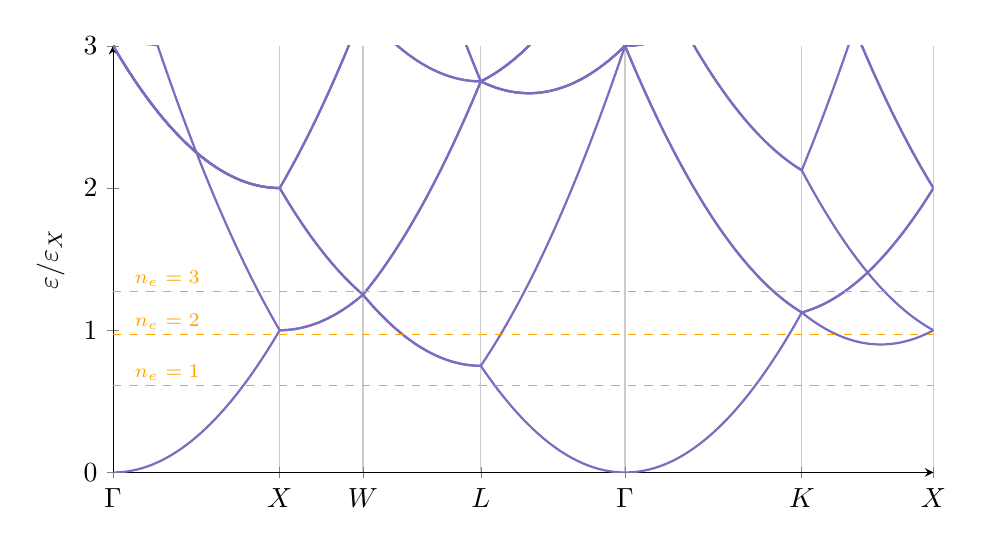
\begin{tikzpicture}
\begin{axis}[
    width=12cm, height=7cm,
    xmin=0, xmax=4.9244, ymin=0, ymax=3,
    ylabel={$\varepsilon/\varepsilon_X$},
    xtick={0.0000,1.0000,1.5000,2.2071,3.0731,4.1338,4.9244},
    xticklabels={$\Gamma$,$X$,$W$,$L$,$\Gamma$,$K$,$X$},
    ytick={0,1,2,3},
    xmajorgrids, grid style={black!20},
    axis lines=left, clip=true,
]
    \addplot[Periwinkle, thick] coordinates {(0.0000,0.0000) (0.0167,0.0003) (0.0333,0.0011) (0.0500,0.0025) (0.0667,0.0044) (0.0833,0.0069) (0.1000,0.0100) (0.1167,0.0136) (0.1333,0.0178) (0.1500,0.0225) (0.1667,0.0278) (0.1833,0.0336) (0.2000,0.0400) (0.2167,0.0469) (0.2333,0.0544) (0.2500,0.0625) (0.2667,0.0711) (0.2833,0.0803) (0.3000,0.0900) (0.3167,0.1003) (0.3333,0.1111) (0.3500,0.1225) (0.3667,0.1344) (0.3833,0.1469) (0.4000,0.1600) (0.4167,0.1736) (0.4333,0.1878) (0.4500,0.2025) (0.4667,0.2178) (0.4833,0.2336) (0.5000,0.2500) (0.5167,0.2669) (0.5333,0.2844) (0.5500,0.3025) (0.5667,0.3211) (0.5833,0.3403) (0.6000,0.3600) (0.6167,0.3803) (0.6333,0.4011) (0.6500,0.4225) (0.6667,0.4444) (0.6833,0.4669) (0.7000,0.4900) (0.7167,0.5136) (0.7333,0.5378) (0.7500,0.5625) (0.7667,0.5878) (0.7833,0.6136) (0.8000,0.6400) (0.8167,0.6669) (0.8333,0.6944) (0.8500,0.7225) (0.8667,0.7511) (0.8833,0.7803) (0.9000,0.8100) (0.9167,0.8403) (0.9333,0.8711) (0.9500,0.9025) (0.9667,0.9344) (0.9833,0.9669) (1.0000,1.0000) (1.0000,1.0000) (1.0083,1.0001) (1.0167,1.0003) (1.0250,1.0006) (1.0333,1.0011) (1.0417,1.0017) (1.0500,1.0025) (1.0583,1.0034) (1.0667,1.0044) (1.0750,1.0056) (1.0833,1.0069) (1.0917,1.0084) (1.1000,1.0100) (1.1083,1.0117) (1.1167,1.0136) (1.1250,1.0156) (1.1333,1.0178) (1.1417,1.0201) (1.1500,1.0225) (1.1583,1.0251) (1.1667,1.0278) (1.1750,1.0306) (1.1833,1.0336) (1.1917,1.0367) (1.2000,1.0400) (1.2083,1.0434) (1.2167,1.0469) (1.2250,1.0506) (1.2333,1.0544) (1.2417,1.0584) (1.2500,1.0625) (1.2583,1.0667) (1.2667,1.0711) (1.2750,1.0756) (1.2833,1.0803) (1.2917,1.0851) (1.3000,1.0900) (1.3083,1.0951) (1.3167,1.1003) (1.3250,1.1056) (1.3333,1.1111) (1.3417,1.1167) (1.3500,1.1225) (1.3583,1.1284) (1.3667,1.1344) (1.3750,1.1406) (1.3833,1.1469) (1.3917,1.1534) (1.4000,1.1600) (1.4083,1.1667) (1.4167,1.1736) (1.4250,1.1806) (1.4333,1.1878) (1.4417,1.1951) (1.4500,1.2025) (1.4583,1.2101) (1.4667,1.2178) (1.4750,1.2256) (1.4833,1.2336) (1.4917,1.2417) (1.5000,1.2500) (1.5000,1.2500) (1.5118,1.2335) (1.5236,1.2172) (1.5354,1.2012) (1.5471,1.1856) (1.5589,1.1701) (1.5707,1.1550) (1.5825,1.1401) (1.5943,1.1256) (1.6061,1.1113) (1.6179,1.0972) (1.6296,1.0835) (1.6414,1.0700) (1.6532,1.0568) (1.6650,1.0439) (1.6768,1.0312) (1.6886,1.0189) (1.7003,1.0068) (1.7121,0.9950) (1.7239,0.9835) (1.7357,0.9722) (1.7475,0.9612) (1.7593,0.9506) (1.7711,0.9401) (1.7828,0.9300) (1.7946,0.9201) (1.8064,0.9106) (1.8182,0.9013) (1.8300,0.8922) (1.8418,0.8835) (1.8536,0.8750) (1.8653,0.8668) (1.8771,0.8589) (1.8889,0.8513) (1.9007,0.8439) (1.9125,0.8368) (1.9243,0.8300) (1.9360,0.8235) (1.9478,0.8172) (1.9596,0.8113) (1.9714,0.8056) (1.9832,0.8001) (1.9950,0.7950) (2.0068,0.7901) (2.0185,0.7856) (2.0303,0.7812) (2.0421,0.7772) (2.0539,0.7735) (2.0657,0.7700) (2.0775,0.7668) (2.0893,0.7639) (2.1010,0.7612) (2.1128,0.7589) (2.1246,0.7568) (2.1364,0.7550) (2.1482,0.7535) (2.1600,0.7522) (2.1718,0.7512) (2.1835,0.7506) (2.1953,0.7501) (2.2071,0.7500) (2.2071,0.7500) (2.2215,0.7252) (2.2360,0.7008) (2.2504,0.6769) (2.2648,0.6533) (2.2793,0.6302) (2.2937,0.6075) (2.3081,0.5852) (2.3226,0.5633) (2.3370,0.5419) (2.3514,0.5208) (2.3659,0.5002) (2.3803,0.4800) (2.3947,0.4602) (2.4092,0.4408) (2.4236,0.4219) (2.4380,0.4033) (2.4525,0.3852) (2.4669,0.3675) (2.4813,0.3502) (2.4958,0.3333) (2.5102,0.3169) (2.5246,0.3008) (2.5391,0.2852) (2.5535,0.2700) (2.5680,0.2552) (2.5824,0.2408) (2.5968,0.2269) (2.6113,0.2133) (2.6257,0.2002) (2.6401,0.1875) (2.6546,0.1752) (2.6690,0.1633) (2.6834,0.1519) (2.6979,0.1408) (2.7123,0.1302) (2.7267,0.1200) (2.7412,0.1102) (2.7556,0.1008) (2.7700,0.0919) (2.7845,0.0833) (2.7989,0.0752) (2.8133,0.0675) (2.8278,0.0602) (2.8422,0.0533) (2.8566,0.0469) (2.8711,0.0408) (2.8855,0.0352) (2.8999,0.0300) (2.9144,0.0252) (2.9288,0.0208) (2.9432,0.0169) (2.9577,0.0133) (2.9721,0.0102) (2.9865,0.0075) (3.0010,0.0052) (3.0154,0.0033) (3.0298,0.0019) (3.0443,0.0008) (3.0587,0.0002) (3.0731,0.0000) (3.0731,0.0000) (3.0908,0.0003) (3.1085,0.0013) (3.1262,0.0028) (3.1438,0.0050) (3.1615,0.0078) (3.1792,0.0113) (3.1969,0.0153) (3.2146,0.0200) (3.2322,0.0253) (3.2499,0.0312) (3.2676,0.0378) (3.2853,0.0450) (3.3029,0.0528) (3.3206,0.0612) (3.3383,0.0703) (3.3560,0.0800) (3.3737,0.0903) (3.3913,0.1012) (3.4090,0.1128) (3.4267,0.1250) (3.4444,0.1378) (3.4620,0.1512) (3.4797,0.1653) (3.4974,0.1800) (3.5151,0.1953) (3.5328,0.2113) (3.5504,0.2278) (3.5681,0.2450) (3.5858,0.2628) (3.6035,0.2812) (3.6211,0.3003) (3.6388,0.3200) (3.6565,0.3403) (3.6742,0.3612) (3.6919,0.3828) (3.7095,0.4050) (3.7272,0.4278) (3.7449,0.4512) (3.7626,0.4753) (3.7802,0.5000) (3.7979,0.5253) (3.8156,0.5512) (3.8333,0.5778) (3.8509,0.6050) (3.8686,0.6328) (3.8863,0.6613) (3.9040,0.6903) (3.9217,0.7200) (3.9393,0.7503) (3.9570,0.7812) (3.9747,0.8128) (3.9924,0.8450) (4.0100,0.8778) (4.0277,0.9113) (4.0454,0.9453) (4.0631,0.9800) (4.0808,1.0153) (4.0984,1.0513) (4.1161,1.0878) (4.1338,1.1250) (4.1338,1.1250) (4.1470,1.1127) (4.1601,1.1007) (4.1733,1.0891) (4.1865,1.0778) (4.1997,1.0668) (4.2128,1.0563) (4.2260,1.0460) (4.2392,1.0361) (4.2524,1.0266) (4.2656,1.0174) (4.2787,1.0085) (4.2919,1.0000) (4.3051,0.9918) (4.3183,0.9840) (4.3314,0.9766) (4.3446,0.9694) (4.3578,0.9627) (4.3710,0.9562) (4.3841,0.9502) (4.3973,0.9444) (4.4105,0.9391) (4.4237,0.9340) (4.4368,0.9293) (4.4500,0.9250) (4.4632,0.9210) (4.4764,0.9174) (4.4895,0.9141) (4.5027,0.9111) (4.5159,0.9085) (4.5291,0.9062) (4.5423,0.9043) (4.5554,0.9028) (4.5686,0.9016) (4.5818,0.9007) (4.5950,0.9002) (4.6081,0.9000) (4.6213,0.9002) (4.6345,0.9007) (4.6477,0.9016) (4.6608,0.9028) (4.6740,0.9043) (4.6872,0.9063) (4.7004,0.9085) (4.7135,0.9111) (4.7267,0.9141) (4.7399,0.9174) (4.7531,0.9210) (4.7662,0.9250) (4.7794,0.9293) (4.7926,0.9340) (4.8058,0.9391) (4.8190,0.9444) (4.8321,0.9502) (4.8453,0.9562) (4.8585,0.9627) (4.8717,0.9694) (4.8848,0.9766) (4.8980,0.9840) (4.9112,0.9918) (4.9244,1.0000)};
    \addplot[Periwinkle, thick] coordinates {(0.0000,3.0000) (0.0167,2.9669) (0.0333,2.9344) (0.0500,2.9025) (0.0667,2.8711) (0.0833,2.8403) (0.1000,2.8100) (0.1167,2.7803) (0.1333,2.7511) (0.1500,2.7225) (0.1667,2.6944) (0.1833,2.6669) (0.2000,2.6400) (0.2167,2.6136) (0.2333,2.5878) (0.2500,2.5625) (0.2667,2.5378) (0.2833,2.5136) (0.3000,2.4900) (0.3167,2.4669) (0.3333,2.4444) (0.3500,2.4225) (0.3667,2.4011) (0.3833,2.3803) (0.4000,2.3600) (0.4167,2.3403) (0.4333,2.3211) (0.4500,2.3025) (0.4667,2.2844) (0.4833,2.2669) (0.5000,2.2500) (0.5167,2.2003) (0.5333,2.1511) (0.5500,2.1025) (0.5667,2.0544) (0.5833,2.0069) (0.6000,1.9600) (0.6167,1.9136) (0.6333,1.8678) (0.6500,1.8225) (0.6667,1.7778) (0.6833,1.7336) (0.7000,1.6900) (0.7167,1.6469) (0.7333,1.6044) (0.7500,1.5625) (0.7667,1.5211) (0.7833,1.4803) (0.8000,1.4400) (0.8167,1.4003) (0.8333,1.3611) (0.8500,1.3225) (0.8667,1.2844) (0.8833,1.2469) (0.9000,1.2100) (0.9167,1.1736) (0.9333,1.1378) (0.9500,1.1025) (0.9667,1.0678) (0.9833,1.0336) (1.0000,1.0000) (1.0000,1.0000) (1.0083,1.0001) (1.0167,1.0003) (1.0250,1.0006) (1.0333,1.0011) (1.0417,1.0017) (1.0500,1.0025) (1.0583,1.0034) (1.0667,1.0044) (1.0750,1.0056) (1.0833,1.0069) (1.0917,1.0084) (1.1000,1.0100) (1.1083,1.0117) (1.1167,1.0136) (1.1250,1.0156) (1.1333,1.0178) (1.1417,1.0201) (1.1500,1.0225) (1.1583,1.0251) (1.1667,1.0278) (1.1750,1.0306) (1.1833,1.0336) (1.1917,1.0367) (1.2000,1.0400) (1.2083,1.0434) (1.2167,1.0469) (1.2250,1.0506) (1.2333,1.0544) (1.2417,1.0584) (1.2500,1.0625) (1.2583,1.0667) (1.2667,1.0711) (1.2750,1.0756) (1.2833,1.0803) (1.2917,1.0851) (1.3000,1.0900) (1.3083,1.0951) (1.3167,1.1003) (1.3250,1.1056) (1.3333,1.1111) (1.3417,1.1167) (1.3500,1.1225) (1.3583,1.1284) (1.3667,1.1344) (1.3750,1.1406) (1.3833,1.1469) (1.3917,1.1534) (1.4000,1.1600) (1.4083,1.1667) (1.4167,1.1736) (1.4250,1.1806) (1.4333,1.1878) (1.4417,1.1951) (1.4500,1.2025) (1.4583,1.2101) (1.4667,1.2178) (1.4750,1.2256) (1.4833,1.2336) (1.4917,1.2417) (1.5000,1.2500) (1.5000,1.2500) (1.5118,1.2335) (1.5236,1.2172) (1.5354,1.2013) (1.5471,1.1856) (1.5589,1.1701) (1.5707,1.1550) (1.5825,1.1401) (1.5943,1.1256) (1.6061,1.1113) (1.6179,1.0972) (1.6296,1.0835) (1.6414,1.0700) (1.6532,1.0568) (1.6650,1.0439) (1.6768,1.0312) (1.6886,1.0189) (1.7003,1.0068) (1.7121,0.9950) (1.7239,0.9835) (1.7357,0.9722) (1.7475,0.9612) (1.7593,0.9506) (1.7711,0.9401) (1.7828,0.9300) (1.7946,0.9201) (1.8064,0.9106) (1.8182,0.9013) (1.8300,0.8922) (1.8418,0.8835) (1.8536,0.8750) (1.8653,0.8668) (1.8771,0.8589) (1.8889,0.8513) (1.9007,0.8439) (1.9125,0.8368) (1.9243,0.8300) (1.9360,0.8235) (1.9478,0.8172) (1.9596,0.8113) (1.9714,0.8056) (1.9832,0.8001) (1.9950,0.7950) (2.0068,0.7901) (2.0185,0.7856) (2.0303,0.7812) (2.0421,0.7772) (2.0539,0.7735) (2.0657,0.7700) (2.0775,0.7668) (2.0893,0.7639) (2.1010,0.7612) (2.1128,0.7589) (2.1246,0.7568) (2.1364,0.7550) (2.1482,0.7535) (2.1600,0.7522) (2.1718,0.7512) (2.1835,0.7506) (2.1953,0.7501) (2.2071,0.7500) (2.2071,0.7500) (2.2215,0.7752) (2.2360,0.8008) (2.2504,0.8269) (2.2648,0.8533) (2.2793,0.8802) (2.2937,0.9075) (2.3081,0.9352) (2.3226,0.9633) (2.3370,0.9919) (2.3514,1.0208) (2.3659,1.0502) (2.3803,1.0800) (2.3947,1.1102) (2.4092,1.1408) (2.4236,1.1719) (2.4380,1.2033) (2.4525,1.2352) (2.4669,1.2675) (2.4813,1.3002) (2.4958,1.3333) (2.5102,1.3669) (2.5246,1.4008) (2.5391,1.4352) (2.5535,1.4700) (2.5680,1.5052) (2.5824,1.5408) (2.5968,1.5769) (2.6113,1.6133) (2.6257,1.6502) (2.6401,1.6875) (2.6546,1.7252) (2.6690,1.7633) (2.6834,1.8019) (2.6979,1.8408) (2.7123,1.8802) (2.7267,1.9200) (2.7412,1.9602) (2.7556,2.0008) (2.7700,2.0419) (2.7845,2.0833) (2.7989,2.1252) (2.8133,2.1675) (2.8278,2.2102) (2.8422,2.2533) (2.8566,2.2969) (2.8711,2.3408) (2.8855,2.3852) (2.8999,2.4300) (2.9144,2.4752) (2.9288,2.5208) (2.9432,2.5669) (2.9577,2.6133) (2.9721,2.6602) (2.9865,2.7075) (3.0010,2.7552) (3.0154,2.8033) (3.0298,2.8519) (3.0443,2.9008) (3.0587,2.9502) (3.0731,3.0000) (3.0731,3.0000) (3.0908,2.9503) (3.1085,2.9013) (3.1262,2.8528) (3.1438,2.8050) (3.1615,2.7578) (3.1792,2.7113) (3.1969,2.6653) (3.2146,2.6200) (3.2322,2.5753) (3.2499,2.5312) (3.2676,2.4878) (3.2853,2.4450) (3.3029,2.4028) (3.3206,2.3613) (3.3383,2.3203) (3.3560,2.2800) (3.3737,2.2403) (3.3913,2.2012) (3.4090,2.1628) (3.4267,2.1250) (3.4444,2.0878) (3.4620,2.0513) (3.4797,2.0153) (3.4974,1.9800) (3.5151,1.9453) (3.5328,1.9113) (3.5504,1.8778) (3.5681,1.8450) (3.5858,1.8128) (3.6035,1.7812) (3.6211,1.7503) (3.6388,1.7200) (3.6565,1.6903) (3.6742,1.6612) (3.6919,1.6328) (3.7095,1.6050) (3.7272,1.5778) (3.7449,1.5513) (3.7626,1.5253) (3.7802,1.5000) (3.7979,1.4753) (3.8156,1.4513) (3.8333,1.4278) (3.8509,1.4050) (3.8686,1.3828) (3.8863,1.3612) (3.9040,1.3403) (3.9217,1.3200) (3.9393,1.3003) (3.9570,1.2812) (3.9747,1.2628) (3.9924,1.2450) (4.0100,1.2278) (4.0277,1.2112) (4.0454,1.1953) (4.0631,1.1800) (4.0808,1.1653) (4.0984,1.1513) (4.1161,1.1378) (4.1338,1.1250) (4.1338,1.1250) (4.1470,1.1293) (4.1601,1.1340) (4.1733,1.1391) (4.1865,1.1444) (4.1997,1.1502) (4.2128,1.1562) (4.2260,1.1627) (4.2392,1.1694) (4.2524,1.1766) (4.2656,1.1840) (4.2787,1.1918) (4.2919,1.2000) (4.3051,1.2085) (4.3183,1.2174) (4.3314,1.2266) (4.3446,1.2361) (4.3578,1.2460) (4.3710,1.2563) (4.3841,1.2668) (4.3973,1.2778) (4.4105,1.2891) (4.4237,1.3007) (4.4368,1.3127) (4.4500,1.3250) (4.4632,1.3377) (4.4764,1.3507) (4.4895,1.3641) (4.5027,1.3778) (4.5159,1.3918) (4.5291,1.4062) (4.5423,1.3877) (4.5554,1.3694) (4.5686,1.3516) (4.5818,1.3340) (4.5950,1.3168) (4.6081,1.3000) (4.6213,1.2835) (4.6345,1.2674) (4.6477,1.2516) (4.6608,1.2361) (4.6740,1.2210) (4.6872,1.2063) (4.7004,1.1918) (4.7135,1.1778) (4.7267,1.1641) (4.7399,1.1507) (4.7531,1.1377) (4.7662,1.1250) (4.7794,1.1127) (4.7926,1.1007) (4.8058,1.0891) (4.8190,1.0778) (4.8321,1.0668) (4.8453,1.0562) (4.8585,1.0460) (4.8717,1.0361) (4.8848,1.0266) (4.8980,1.0174) (4.9112,1.0085) (4.9244,1.0000)};
    \addplot[Periwinkle, thick] coordinates {(0.0000,3.0000) (0.0167,2.9669) (0.0333,2.9344) (0.0500,2.9025) (0.0667,2.8711) (0.0833,2.8403) (0.1000,2.8100) (0.1167,2.7803) (0.1333,2.7511) (0.1500,2.7225) (0.1667,2.6944) (0.1833,2.6669) (0.2000,2.6400) (0.2167,2.6136) (0.2333,2.5878) (0.2500,2.5625) (0.2667,2.5378) (0.2833,2.5136) (0.3000,2.4900) (0.3167,2.4669) (0.3333,2.4444) (0.3500,2.4225) (0.3667,2.4011) (0.3833,2.3803) (0.4000,2.3600) (0.4167,2.3403) (0.4333,2.3211) (0.4500,2.3025) (0.4667,2.2844) (0.4833,2.2669) (0.5000,2.2500) (0.5167,2.2336) (0.5333,2.2178) (0.5500,2.2025) (0.5667,2.1878) (0.5833,2.1736) (0.6000,2.1600) (0.6167,2.1469) (0.6333,2.1344) (0.6500,2.1225) (0.6667,2.1111) (0.6833,2.1003) (0.7000,2.0900) (0.7167,2.0803) (0.7333,2.0711) (0.7500,2.0625) (0.7667,2.0544) (0.7833,2.0469) (0.8000,2.0400) (0.8167,2.0336) (0.8333,2.0278) (0.8500,2.0225) (0.8667,2.0178) (0.8833,2.0136) (0.9000,2.0100) (0.9167,2.0069) (0.9333,2.0044) (0.9500,2.0025) (0.9667,2.0011) (0.9833,2.0003) (1.0000,2.0000) (1.0000,2.0000) (1.0083,1.9834) (1.0167,1.9669) (1.0250,1.9506) (1.0333,1.9344) (1.0417,1.9184) (1.0500,1.9025) (1.0583,1.8867) (1.0667,1.8711) (1.0750,1.8556) (1.0833,1.8403) (1.0917,1.8251) (1.1000,1.8100) (1.1083,1.7951) (1.1167,1.7803) (1.1250,1.7656) (1.1333,1.7511) (1.1417,1.7367) (1.1500,1.7225) (1.1583,1.7084) (1.1667,1.6944) (1.1750,1.6806) (1.1833,1.6669) (1.1917,1.6534) (1.2000,1.6400) (1.2083,1.6267) (1.2167,1.6136) (1.2250,1.6006) (1.2333,1.5878) (1.2417,1.5751) (1.2500,1.5625) (1.2583,1.5501) (1.2667,1.5378) (1.2750,1.5256) (1.2833,1.5136) (1.2917,1.5017) (1.3000,1.4900) (1.3083,1.4784) (1.3167,1.4669) (1.3250,1.4556) (1.3333,1.4444) (1.3417,1.4334) (1.3500,1.4225) (1.3583,1.4117) (1.3667,1.4011) (1.3750,1.3906) (1.3833,1.3803) (1.3917,1.3701) (1.4000,1.3600) (1.4083,1.3501) (1.4167,1.3403) (1.4250,1.3306) (1.4333,1.3211) (1.4417,1.3117) (1.4500,1.3025) (1.4583,1.2934) (1.4667,1.2844) (1.4750,1.2756) (1.4833,1.2669) (1.4917,1.2584) (1.5000,1.2500) (1.5000,1.2500) (1.5118,1.2668) (1.5236,1.2839) (1.5354,1.3013) (1.5471,1.3189) (1.5589,1.3368) (1.5707,1.3550) (1.5825,1.3735) (1.5943,1.3922) (1.6061,1.4112) (1.6179,1.4306) (1.6296,1.4501) (1.6414,1.4700) (1.6532,1.4901) (1.6650,1.5106) (1.6768,1.5312) (1.6886,1.5522) (1.7003,1.5735) (1.7121,1.5950) (1.7239,1.6168) (1.7357,1.6389) (1.7475,1.6613) (1.7593,1.6839) (1.7711,1.7068) (1.7828,1.7300) (1.7946,1.7535) (1.8064,1.7772) (1.8182,1.8013) (1.8300,1.8256) (1.8418,1.8501) (1.8536,1.8750) (1.8653,1.9001) (1.8771,1.9256) (1.8889,1.9512) (1.9007,1.9772) (1.9125,2.0035) (1.9243,2.0300) (1.9360,2.0568) (1.9478,2.0839) (1.9596,2.1113) (1.9714,2.1389) (1.9832,2.1668) (1.9950,2.1950) (2.0068,2.2235) (2.0185,2.2522) (2.0303,2.2812) (2.0421,2.3106) (2.0539,2.3401) (2.0657,2.3700) (2.0775,2.4001) (2.0893,2.4306) (2.1010,2.4613) (2.1128,2.4922) (2.1246,2.5235) (2.1364,2.5550) (2.1482,2.5868) (2.1600,2.6189) (2.1718,2.6513) (2.1835,2.6839) (2.1953,2.7168) (2.2071,2.7500) (2.2071,2.7500) (2.2215,2.7419) (2.2360,2.7342) (2.2504,2.7269) (2.2648,2.7200) (2.2793,2.7135) (2.2937,2.7075) (2.3081,2.7019) (2.3226,2.6967) (2.3370,2.6919) (2.3514,2.6875) (2.3659,2.6835) (2.3803,2.6800) (2.3947,2.6769) (2.4092,2.6742) (2.4236,2.6719) (2.4380,2.6700) (2.4525,2.6685) (2.4669,2.6675) (2.4813,2.6669) (2.4958,2.6667) (2.5102,2.6669) (2.5246,2.6675) (2.5391,2.6685) (2.5535,2.6700) (2.5680,2.6719) (2.5824,2.6742) (2.5968,2.6769) (2.6113,2.6800) (2.6257,2.6835) (2.6401,2.6875) (2.6546,2.6919) (2.6690,2.6967) (2.6834,2.7019) (2.6979,2.7075) (2.7123,2.7135) (2.7267,2.7200) (2.7412,2.7269) (2.7556,2.7342) (2.7700,2.7419) (2.7845,2.7500) (2.7989,2.7585) (2.8133,2.7675) (2.8278,2.7769) (2.8422,2.7867) (2.8566,2.7969) (2.8711,2.8075) (2.8855,2.8185) (2.8999,2.8300) (2.9144,2.8419) (2.9288,2.8542) (2.9432,2.8669) (2.9577,2.8800) (2.9721,2.8935) (2.9865,2.9075) (3.0010,2.9219) (3.0154,2.9367) (3.0298,2.9519) (3.0443,2.9675) (3.0587,2.9835) (3.0731,3.0000) (3.0731,3.0000) (3.0908,2.9503) (3.1085,2.9013) (3.1262,2.8528) (3.1438,2.8050) (3.1615,2.7578) (3.1792,2.7113) (3.1969,2.6653) (3.2146,2.6200) (3.2322,2.5753) (3.2499,2.5312) (3.2676,2.4878) (3.2853,2.4450) (3.3029,2.4028) (3.3206,2.3613) (3.3383,2.3203) (3.3560,2.2800) (3.3737,2.2403) (3.3913,2.2012) (3.4090,2.1628) (3.4267,2.1250) (3.4444,2.0878) (3.4620,2.0513) (3.4797,2.0153) (3.4974,1.9800) (3.5151,1.9453) (3.5328,1.9113) (3.5504,1.8778) (3.5681,1.8450) (3.5858,1.8128) (3.6035,1.7812) (3.6211,1.7503) (3.6388,1.7200) (3.6565,1.6903) (3.6742,1.6612) (3.6919,1.6328) (3.7095,1.6050) (3.7272,1.5778) (3.7449,1.5513) (3.7626,1.5253) (3.7802,1.5000) (3.7979,1.4753) (3.8156,1.4513) (3.8333,1.4278) (3.8509,1.4050) (3.8686,1.3828) (3.8863,1.3612) (3.9040,1.3403) (3.9217,1.3200) (3.9393,1.3003) (3.9570,1.2812) (3.9747,1.2628) (3.9924,1.2450) (4.0100,1.2278) (4.0277,1.2112) (4.0454,1.1953) (4.0631,1.1800) (4.0808,1.1653) (4.0984,1.1513) (4.1161,1.1378) (4.1338,1.1250) (4.1338,1.1250) (4.1470,1.1293) (4.1601,1.1340) (4.1733,1.1391) (4.1865,1.1444) (4.1997,1.1502) (4.2128,1.1562) (4.2260,1.1627) (4.2392,1.1694) (4.2524,1.1766) (4.2656,1.1840) (4.2787,1.1918) (4.2919,1.2000) (4.3051,1.2085) (4.3183,1.2174) (4.3314,1.2266) (4.3446,1.2361) (4.3578,1.2460) (4.3710,1.2563) (4.3841,1.2668) (4.3973,1.2778) (4.4105,1.2891) (4.4237,1.3007) (4.4368,1.3127) (4.4500,1.3250) (4.4632,1.3377) (4.4764,1.3507) (4.4895,1.3641) (4.5027,1.3778) (4.5159,1.3918) (4.5291,1.4062) (4.5423,1.4210) (4.5554,1.4361) (4.5686,1.4516) (4.5818,1.4674) (4.5950,1.4835) (4.6081,1.5000) (4.6213,1.5168) (4.6345,1.5340) (4.6477,1.5516) (4.6608,1.5694) (4.6740,1.5877) (4.6872,1.6062) (4.7004,1.6252) (4.7135,1.6444) (4.7267,1.6641) (4.7399,1.6840) (4.7531,1.7043) (4.7662,1.7250) (4.7794,1.7460) (4.7926,1.7674) (4.8058,1.7891) (4.8190,1.8111) (4.8321,1.8335) (4.8453,1.8563) (4.8585,1.8793) (4.8717,1.9028) (4.8848,1.9266) (4.8980,1.9507) (4.9112,1.9752) (4.9244,2.0000)};
    \addplot[Periwinkle, thick] coordinates {(0.0000,3.0000) (0.0167,2.9669) (0.0333,2.9344) (0.0500,2.9025) (0.0667,2.8711) (0.0833,2.8403) (0.1000,2.8100) (0.1167,2.7803) (0.1333,2.7511) (0.1500,2.7225) (0.1667,2.6944) (0.1833,2.6669) (0.2000,2.6400) (0.2167,2.6136) (0.2333,2.5878) (0.2500,2.5625) (0.2667,2.5378) (0.2833,2.5136) (0.3000,2.4900) (0.3167,2.4669) (0.3333,2.4444) (0.3500,2.4225) (0.3667,2.4011) (0.3833,2.3803) (0.4000,2.3600) (0.4167,2.3403) (0.4333,2.3211) (0.4500,2.3025) (0.4667,2.2844) (0.4833,2.2669) (0.5000,2.2500) (0.5167,2.2336) (0.5333,2.2178) (0.5500,2.2025) (0.5667,2.1878) (0.5833,2.1736) (0.6000,2.1600) (0.6167,2.1469) (0.6333,2.1344) (0.6500,2.1225) (0.6667,2.1111) (0.6833,2.1003) (0.7000,2.0900) (0.7167,2.0803) (0.7333,2.0711) (0.7500,2.0625) (0.7667,2.0544) (0.7833,2.0469) (0.8000,2.0400) (0.8167,2.0336) (0.8333,2.0278) (0.8500,2.0225) (0.8667,2.0178) (0.8833,2.0136) (0.9000,2.0100) (0.9167,2.0069) (0.9333,2.0044) (0.9500,2.0025) (0.9667,2.0011) (0.9833,2.0003) (1.0000,2.0000) (1.0000,2.0000) (1.0083,1.9834) (1.0167,1.9669) (1.0250,1.9506) (1.0333,1.9344) (1.0417,1.9184) (1.0500,1.9025) (1.0583,1.8867) (1.0667,1.8711) (1.0750,1.8556) (1.0833,1.8403) (1.0917,1.8251) (1.1000,1.8100) (1.1083,1.7951) (1.1167,1.7803) (1.1250,1.7656) (1.1333,1.7511) (1.1417,1.7367) (1.1500,1.7225) (1.1583,1.7084) (1.1667,1.6944) (1.1750,1.6806) (1.1833,1.6669) (1.1917,1.6534) (1.2000,1.6400) (1.2083,1.6267) (1.2167,1.6136) (1.2250,1.6006) (1.2333,1.5878) (1.2417,1.5751) (1.2500,1.5625) (1.2583,1.5501) (1.2667,1.5378) (1.2750,1.5256) (1.2833,1.5136) (1.2917,1.5017) (1.3000,1.4900) (1.3083,1.4784) (1.3167,1.4669) (1.3250,1.4556) (1.3333,1.4444) (1.3417,1.4334) (1.3500,1.4225) (1.3583,1.4117) (1.3667,1.4011) (1.3750,1.3906) (1.3833,1.3803) (1.3917,1.3701) (1.4000,1.3600) (1.4083,1.3501) (1.4167,1.3403) (1.4250,1.3306) (1.4333,1.3211) (1.4417,1.3117) (1.4500,1.3025) (1.4583,1.2934) (1.4667,1.2844) (1.4750,1.2756) (1.4833,1.2669) (1.4917,1.2584) (1.5000,1.2500) (1.5000,1.2500) (1.5118,1.2668) (1.5236,1.2839) (1.5354,1.3013) (1.5471,1.3189) (1.5589,1.3368) (1.5707,1.3550) (1.5825,1.3735) (1.5943,1.3922) (1.6061,1.4112) (1.6179,1.4306) (1.6296,1.4501) (1.6414,1.4700) (1.6532,1.4901) (1.6650,1.5106) (1.6768,1.5312) (1.6886,1.5522) (1.7003,1.5735) (1.7121,1.5950) (1.7239,1.6168) (1.7357,1.6389) (1.7475,1.6613) (1.7593,1.6839) (1.7711,1.7068) (1.7828,1.7300) (1.7946,1.7535) (1.8064,1.7772) (1.8182,1.8013) (1.8300,1.8256) (1.8418,1.8501) (1.8536,1.8750) (1.8653,1.9001) (1.8771,1.9256) (1.8889,1.9512) (1.9007,1.9772) (1.9125,2.0035) (1.9243,2.0300) (1.9360,2.0568) (1.9478,2.0839) (1.9596,2.1113) (1.9714,2.1389) (1.9832,2.1668) (1.9950,2.1950) (2.0068,2.2235) (2.0185,2.2522) (2.0303,2.2812) (2.0421,2.3106) (2.0539,2.3401) (2.0657,2.3700) (2.0775,2.4001) (2.0893,2.4306) (2.1010,2.4613) (2.1128,2.4922) (2.1246,2.5235) (2.1364,2.5550) (2.1482,2.5868) (2.1600,2.6189) (2.1718,2.6513) (2.1835,2.6839) (2.1953,2.7168) (2.2071,2.7500) (2.2071,2.7500) (2.2215,2.7419) (2.2360,2.7342) (2.2504,2.7269) (2.2648,2.7200) (2.2793,2.7135) (2.2937,2.7075) (2.3081,2.7019) (2.3226,2.6967) (2.3370,2.6919) (2.3514,2.6875) (2.3659,2.6835) (2.3803,2.6800) (2.3947,2.6769) (2.4092,2.6742) (2.4236,2.6719) (2.4380,2.6700) (2.4525,2.6685) (2.4669,2.6675) (2.4813,2.6669) (2.4958,2.6667) (2.5102,2.6669) (2.5246,2.6675) (2.5391,2.6685) (2.5535,2.6700) (2.5680,2.6719) (2.5824,2.6742) (2.5968,2.6769) (2.6113,2.6800) (2.6257,2.6835) (2.6401,2.6875) (2.6546,2.6919) (2.6690,2.6967) (2.6834,2.7019) (2.6979,2.7075) (2.7123,2.7135) (2.7267,2.7200) (2.7412,2.7269) (2.7556,2.7342) (2.7700,2.7419) (2.7845,2.7500) (2.7989,2.7585) (2.8133,2.7675) (2.8278,2.7769) (2.8422,2.7867) (2.8566,2.7969) (2.8711,2.8075) (2.8855,2.8185) (2.8999,2.8300) (2.9144,2.8419) (2.9288,2.8542) (2.9432,2.8669) (2.9577,2.8800) (2.9721,2.8935) (2.9865,2.9075) (3.0010,2.9219) (3.0154,2.9367) (3.0298,2.9519) (3.0443,2.9675) (3.0587,2.9835) (3.0731,3.0000) (3.0731,3.0000) (3.0908,3.0003) (3.1085,3.0012) (3.1262,3.0028) (3.1438,3.0050) (3.1615,3.0078) (3.1792,3.0112) (3.1969,3.0153) (3.2146,3.0200) (3.2322,3.0253) (3.2499,3.0312) (3.2676,3.0378) (3.2853,3.0450) (3.4797,3.0153) (3.4974,2.9800) (3.5151,2.9453) (3.5328,2.9112) (3.5504,2.8778) (3.5681,2.8450) (3.5858,2.8128) (3.6035,2.7812) (3.6211,2.7503) (3.6388,2.7200) (3.6565,2.6903) (3.6742,2.6612) (3.6919,2.6328) (3.7095,2.6050) (3.7272,2.5778) (3.7449,2.5512) (3.7626,2.5253) (3.7802,2.5000) (3.7979,2.4753) (3.8156,2.4512) (3.8333,2.4278) (3.8509,2.4050) (3.8686,2.3828) (3.8863,2.3612) (3.9040,2.3403) (3.9217,2.3200) (3.9393,2.3003) (3.9570,2.2812) (3.9747,2.2628) (3.9924,2.2450) (4.0100,2.2278) (4.0277,2.2113) (4.0454,2.1953) (4.0631,2.1800) (4.0808,2.1653) (4.0984,2.1513) (4.1161,2.1378) (4.1338,2.1250) (4.1338,2.1250) (4.1470,2.0960) (4.1601,2.0674) (4.1733,2.0391) (4.1865,2.0111) (4.1997,1.9835) (4.2128,1.9563) (4.2260,1.9293) (4.2392,1.9028) (4.2524,1.8766) (4.2656,1.8507) (4.2787,1.8252) (4.2919,1.8000) (4.3051,1.7752) (4.3183,1.7507) (4.3314,1.7266) (4.3446,1.7028) (4.3578,1.6793) (4.3710,1.6563) (4.3841,1.6335) (4.3973,1.6111) (4.4105,1.5891) (4.4237,1.5674) (4.4368,1.5460) (4.4500,1.5250) (4.4632,1.5043) (4.4764,1.4840) (4.4895,1.4641) (4.5027,1.4444) (4.5159,1.4252) (4.5291,1.4062) (4.5423,1.4210) (4.5554,1.4361) (4.5686,1.4516) (4.5818,1.4674) (4.5950,1.4835) (4.6081,1.5000) (4.6213,1.5168) (4.6345,1.5340) (4.6477,1.5516) (4.6608,1.5694) (4.6740,1.5877) (4.6872,1.6062) (4.7004,1.6252) (4.7135,1.6444) (4.7267,1.6641) (4.7399,1.6840) (4.7531,1.7043) (4.7662,1.7250) (4.7794,1.7460) (4.7926,1.7674) (4.8058,1.7891) (4.8190,1.8111) (4.8321,1.8335) (4.8453,1.8563) (4.8585,1.8793) (4.8717,1.9028) (4.8848,1.9266) (4.8980,1.9507) (4.9112,1.9752) (4.9244,2.0000)};
    \addplot[Periwinkle, thick] coordinates {(0.0000,3.0000) (0.0167,2.9669) (0.0333,2.9344) (0.0500,2.9025) (0.0667,2.8711) (0.0833,2.8403) (0.1000,2.8100) (0.1167,2.7803) (0.1333,2.7511) (0.1500,2.7225) (0.1667,2.6944) (0.1833,2.6669) (0.2000,2.6400) (0.2167,2.6136) (0.2333,2.5878) (0.2500,2.5625) (0.2667,2.5378) (0.2833,2.5136) (0.3000,2.4900) (0.3167,2.4669) (0.3333,2.4444) (0.3500,2.4225) (0.3667,2.4011) (0.3833,2.3803) (0.4000,2.3600) (0.4167,2.3403) (0.4333,2.3211) (0.4500,2.3025) (0.4667,2.2844) (0.4833,2.2669) (0.5000,2.2500) (0.5167,2.2336) (0.5333,2.2178) (0.5500,2.2025) (0.5667,2.1878) (0.5833,2.1736) (0.6000,2.1600) (0.6167,2.1469) (0.6333,2.1344) (0.6500,2.1225) (0.6667,2.1111) (0.6833,2.1003) (0.7000,2.0900) (0.7167,2.0803) (0.7333,2.0711) (0.7500,2.0625) (0.7667,2.0544) (0.7833,2.0469) (0.8000,2.0400) (0.8167,2.0336) (0.8333,2.0278) (0.8500,2.0225) (0.8667,2.0178) (0.8833,2.0136) (0.9000,2.0100) (0.9167,2.0069) (0.9333,2.0044) (0.9500,2.0025) (0.9667,2.0011) (0.9833,2.0003) (1.0000,2.0000) (1.0000,2.0000) (1.0083,2.0167) (1.0167,2.0336) (1.0250,2.0506) (1.0333,2.0678) (1.0417,2.0851) (1.0500,2.1025) (1.0583,2.1201) (1.0667,2.1378) (1.0750,2.1556) (1.0833,2.1736) (1.0917,2.1917) (1.1000,2.2100) (1.1083,2.2284) (1.1167,2.2469) (1.1250,2.2656) (1.1333,2.2844) (1.1417,2.3034) (1.1500,2.3225) (1.1583,2.3417) (1.1667,2.3611) (1.1750,2.3806) (1.1833,2.4003) (1.1917,2.4201) (1.2000,2.4400) (1.2083,2.4601) (1.2167,2.4803) (1.2250,2.5006) (1.2333,2.5211) (1.2417,2.5417) (1.2500,2.5625) (1.2583,2.5834) (1.2667,2.6044) (1.2750,2.6256) (1.2833,2.6469) (1.2917,2.6684) (1.3000,2.6900) (1.3083,2.7117) (1.3167,2.7336) (1.3250,2.7556) (1.3333,2.7778) (1.3417,2.8001) (1.3500,2.8225) (1.3583,2.8451) (1.3667,2.8678) (1.3750,2.8906) (1.3833,2.9136) (1.3917,2.9367) (1.4000,2.9600) (1.4083,2.9834) (1.4167,3.0069) (1.4250,3.0306) (1.6650,3.0439) (1.6768,3.0312) (1.6886,3.0189) (1.7003,3.0068) (1.7121,2.9950) (1.7239,2.9835) (1.7357,2.9722) (1.7475,2.9613) (1.7593,2.9506) (1.7711,2.9401) (1.7828,2.9300) (1.7946,2.9201) (1.8064,2.9106) (1.8182,2.9013) (1.8300,2.8922) (1.8418,2.8835) (1.8536,2.8750) (1.8653,2.8668) (1.8771,2.8589) (1.8889,2.8512) (1.9007,2.8439) (1.9125,2.8368) (1.9243,2.8300) (1.9360,2.8235) (1.9478,2.8172) (1.9596,2.8112) (1.9714,2.8056) (1.9832,2.8001) (1.9950,2.7950) (2.0068,2.7901) (2.0185,2.7856) (2.0303,2.7812) (2.0421,2.7772) (2.0539,2.7735) (2.0657,2.7700) (2.0775,2.7668) (2.0893,2.7639) (2.1010,2.7612) (2.1128,2.7589) (2.1246,2.7568) (2.1364,2.7550) (2.1482,2.7535) (2.1600,2.7522) (2.1718,2.7512) (2.1835,2.7506) (2.1953,2.7501) (2.2071,2.7500) (2.2071,2.7500) (2.2215,2.7419) (2.2360,2.7342) (2.2504,2.7269) (2.2648,2.7200) (2.2793,2.7135) (2.2937,2.7075) (2.3081,2.7019) (2.3226,2.6967) (2.3370,2.6919) (2.3514,2.6875) (2.3659,2.6835) (2.3803,2.6800) (2.3947,2.6769) (2.4092,2.6742) (2.4236,2.6719) (2.4380,2.6700) (2.4525,2.6685) (2.4669,2.6675) (2.4813,2.6669) (2.4958,2.6667) (2.5102,2.6669) (2.5246,2.6675) (2.5391,2.6685) (2.5535,2.6700) (2.5680,2.6719) (2.5824,2.6742) (2.5968,2.6769) (2.6113,2.6800) (2.6257,2.6835) (2.6401,2.6875) (2.6546,2.6919) (2.6690,2.6967) (2.6834,2.7019) (2.6979,2.7075) (2.7123,2.7135) (2.7267,2.7200) (2.7412,2.7269) (2.7556,2.7342) (2.7700,2.7419) (2.7845,2.7500) (2.7989,2.7585) (2.8133,2.7675) (2.8278,2.7769) (2.8422,2.7867) (2.8566,2.7969) (2.8711,2.8075) (2.8855,2.8185) (2.8999,2.8300) (2.9144,2.8419) (2.9288,2.8542) (2.9432,2.8669) (2.9577,2.8800) (2.9721,2.8935) (2.9865,2.9075) (3.0010,2.9219) (3.0154,2.9367) (3.0298,2.9519) (3.0443,2.9675) (3.0587,2.9835) (3.0731,3.0000) (3.0731,3.0000) (3.0908,3.0003) (3.1085,3.0012) (3.1262,3.0028) (3.1438,3.0050) (3.1615,3.0078) (3.1792,3.0112) (3.1969,3.0153) (3.2146,3.0200) (3.2322,3.0253) (3.2499,3.0312) (3.2676,3.0378) (3.2853,3.0450) (3.4797,3.0153) (3.4974,2.9800) (3.5151,2.9453) (3.5328,2.9112) (3.5504,2.8778) (3.5681,2.8450) (3.5858,2.8128) (3.6035,2.7812) (3.6211,2.7503) (3.6388,2.7200) (3.6565,2.6903) (3.6742,2.6612) (3.6919,2.6328) (3.7095,2.6050) (3.7272,2.5778) (3.7449,2.5512) (3.7626,2.5253) (3.7802,2.5000) (3.7979,2.4753) (3.8156,2.4512) (3.8333,2.4278) (3.8509,2.4050) (3.8686,2.3828) (3.8863,2.3612) (3.9040,2.3403) (3.9217,2.3200) (3.9393,2.3003) (3.9570,2.2812) (3.9747,2.2628) (3.9924,2.2450) (4.0100,2.2278) (4.0277,2.2113) (4.0454,2.1953) (4.0631,2.1800) (4.0808,2.1653) (4.0984,2.1513) (4.1161,2.1378) (4.1338,2.1250) (4.1338,2.1250) (4.1470,2.1627) (4.1601,2.2007) (4.1733,2.2391) (4.1865,2.2778) (4.1997,2.3168) (4.2128,2.3563) (4.2260,2.3960) (4.2392,2.4361) (4.2524,2.4766) (4.2656,2.5174) (4.2787,2.5585) (4.2919,2.6000) (4.3051,2.6418) (4.3183,2.6840) (4.3314,2.7266) (4.3446,2.7694) (4.3578,2.8127) (4.3710,2.8563) (4.3841,2.9002) (4.3973,2.9444) (4.4105,2.9891) (4.4237,3.0340) (4.4895,3.0141) (4.5027,2.9778) (4.5159,2.9418) (4.5291,2.9062) (4.5423,2.8710) (4.5554,2.8361) (4.5686,2.8016) (4.5818,2.7674) (4.5950,2.7335) (4.6081,2.7000) (4.6213,2.6668) (4.6345,2.6340) (4.6477,2.6016) (4.6608,2.5694) (4.6740,2.5377) (4.6872,2.5063) (4.7004,2.4752) (4.7135,2.4444) (4.7267,2.4141) (4.7399,2.3840) (4.7531,2.3543) (4.7662,2.3250) (4.7794,2.2960) (4.7926,2.2674) (4.8058,2.2391) (4.8190,2.2111) (4.8321,2.1835) (4.8453,2.1562) (4.8585,2.1293) (4.8717,2.1028) (4.8848,2.0766) (4.8980,2.0507) (4.9112,2.0252) (4.9244,2.0000)};
    \addplot[Periwinkle, thick] coordinates {(0.0000,3.0000) (0.0167,3.0336) (0.2667,3.0044) (0.2833,2.9469) (0.3000,2.8900) (0.3167,2.8336) (0.3333,2.7778) (0.3500,2.7225) (0.3667,2.6678) (0.3833,2.6136) (0.4000,2.5600) (0.4167,2.5069) (0.4333,2.4544) (0.4500,2.4025) (0.4667,2.3511) (0.4833,2.3003) (0.5000,2.2500) (0.5167,2.2336) (0.5333,2.2178) (0.5500,2.2025) (0.5667,2.1878) (0.5833,2.1736) (0.6000,2.1600) (0.6167,2.1469) (0.6333,2.1344) (0.6500,2.1225) (0.6667,2.1111) (0.6833,2.1003) (0.7000,2.0900) (0.7167,2.0803) (0.7333,2.0711) (0.7500,2.0625) (0.7667,2.0544) (0.7833,2.0469) (0.8000,2.0400) (0.8167,2.0336) (0.8333,2.0278) (0.8500,2.0225) (0.8667,2.0178) (0.8833,2.0136) (0.9000,2.0100) (0.9167,2.0069) (0.9333,2.0044) (0.9500,2.0025) (0.9667,2.0011) (0.9833,2.0003) (1.0000,2.0000) (1.0000,2.0000) (1.0083,2.0167) (1.0167,2.0336) (1.0250,2.0506) (1.0333,2.0678) (1.0417,2.0851) (1.0500,2.1025) (1.0583,2.1201) (1.0667,2.1378) (1.0750,2.1556) (1.0833,2.1736) (1.0917,2.1917) (1.1000,2.2100) (1.1083,2.2284) (1.1167,2.2469) (1.1250,2.2656) (1.1333,2.2844) (1.1417,2.3034) (1.1500,2.3225) (1.1583,2.3417) (1.1667,2.3611) (1.1750,2.3806) (1.1833,2.4003) (1.1917,2.4201) (1.2000,2.4400) (1.2083,2.4601) (1.2167,2.4803) (1.2250,2.5006) (1.2333,2.5211) (1.2417,2.5417) (1.2500,2.5625) (1.2583,2.5834) (1.2667,2.6044) (1.2750,2.6256) (1.2833,2.6469) (1.2917,2.6684) (1.3000,2.6900) (1.3083,2.7117) (1.3167,2.7336) (1.3250,2.7556) (1.3333,2.7778) (1.3417,2.8001) (1.3500,2.8225) (1.3583,2.8451) (1.3667,2.8678) (1.3750,2.8906) (1.3833,2.9136) (1.3917,2.9367) (1.4000,2.9600) (1.4083,2.9834) (1.4167,3.0069) (1.4250,3.0306) (1.6650,3.0439) (1.6768,3.0312) (1.6886,3.0189) (1.7003,3.0068) (1.7121,2.9950) (1.7239,2.9835) (1.7357,2.9722) (1.7475,2.9613) (1.7593,2.9506) (1.7711,2.9401) (1.7828,2.9300) (1.7946,2.9201) (1.8064,2.9106) (1.8182,2.9013) (1.8300,2.8922) (1.8418,2.8835) (1.8536,2.8750) (1.8653,2.8668) (1.8771,2.8589) (1.8889,2.8513) (1.9007,2.8439) (1.9125,2.8368) (1.9243,2.8300) (1.9360,2.8235) (1.9478,2.8172) (1.9596,2.8112) (1.9714,2.8056) (1.9832,2.8001) (1.9950,2.7950) (2.0068,2.7901) (2.0185,2.7856) (2.0303,2.7812) (2.0421,2.7772) (2.0539,2.7735) (2.0657,2.7700) (2.0775,2.7668) (2.0893,2.7639) (2.1010,2.7612) (2.1128,2.7589) (2.1246,2.7568) (2.1364,2.7550) (2.1482,2.7535) (2.1600,2.7522) (2.1718,2.7512) (2.1835,2.7506) (2.1953,2.7501) (2.2071,2.7500) (2.2071,2.7500) (2.2215,2.7585) (2.2360,2.7675) (2.2504,2.7769) (2.2648,2.7867) (2.2793,2.7969) (2.2937,2.8075) (2.3081,2.8185) (2.3226,2.8300) (2.3370,2.8419) (2.3514,2.8542) (2.3659,2.8669) (2.3803,2.8800) (2.3947,2.8935) (2.4092,2.9075) (2.4236,2.9219) (2.4380,2.9367) (2.4525,2.9519) (2.4669,2.9675) (2.4813,2.9835) (2.4958,3.0000) (2.5102,3.0169) (2.5246,3.0342) (3.0443,3.0342) (3.0587,3.0169) (3.0731,3.0000) (3.0731,3.0000) (3.0908,3.0003) (3.1085,3.0012) (3.1262,3.0028) (3.1438,3.0050) (3.1615,3.0078) (3.1792,3.0112) (3.1969,3.0153) (3.2146,3.0200) (3.2322,3.0253) (3.2499,3.0312) (3.2676,3.0378) (3.2853,3.0450) (4.4895,3.0141) (4.5027,2.9778) (4.5159,2.9418) (4.5291,2.9062) (4.5423,2.8710) (4.5554,2.8361) (4.5686,2.8016) (4.5818,2.7674) (4.5950,2.7335) (4.6081,2.7000) (4.6213,2.6668) (4.6345,2.6340) (4.6477,2.6016) (4.6608,2.5694) (4.6740,2.5377) (4.6872,2.5063) (4.7004,2.4752) (4.7135,2.4444) (4.7267,2.4141) (4.7399,2.3840) (4.7531,2.3543) (4.7662,2.3250) (4.7794,2.2960) (4.7926,2.2674) (4.8058,2.2391) (4.8190,2.2111) (4.8321,2.1835) (4.8453,2.1562) (4.8585,2.1293) (4.8717,2.1028) (4.8848,2.0766) (4.8980,2.0507) (4.9112,2.0252) (4.9244,2.0000)};
    \addplot[Periwinkle, thick] coordinates {(0.0000,3.0000) (0.0167,3.0336) (2.1128,3.0256) (2.1246,2.9901) (2.1364,2.9550) (2.1482,2.9201) (2.1600,2.8856) (2.1718,2.8512) (2.1835,2.8172) (2.1953,2.7835) (2.2071,2.7500) (2.2071,2.7500) (2.2215,2.7585) (2.2360,2.7675) (2.2504,2.7769) (2.2648,2.7867) (2.2793,2.7969) (2.2937,2.8075) (2.3081,2.8185) (2.3226,2.8300) (2.3370,2.8419) (2.3514,2.8542) (2.3659,2.8669) (2.3803,2.8800) (2.3947,2.8935) (2.4092,2.9075) (2.4236,2.9219) (2.4380,2.9367) (2.4525,2.9519) (2.4669,2.9675) (2.4813,2.9835) (2.4958,3.0000) (2.5102,3.0169) (2.5246,3.0342) (3.0443,3.0342) (3.0587,3.0169) (3.0731,3.0000) (3.0731,3.0000) (3.0908,3.0003) (3.1085,3.0012) (3.1262,3.0028) (3.1438,3.0050) (3.1615,3.0078) (3.1792,3.0112) (3.1969,3.0153) (3.2146,3.0200) (3.2322,3.0253) (3.2499,3.0312) (3.2676,3.0378) (3.2853,3.0450)};
    \addplot[Periwinkle, thick] coordinates {(0.0000,3.0000) (0.0167,3.0336) (2.1128,3.0256) (2.1246,2.9901) (2.1364,2.9550) (2.1482,2.9201) (2.1600,2.8856) (2.1718,2.8512) (2.1835,2.8172) (2.1953,2.7835) (2.2071,2.7500) (2.2071,2.7500) (2.2215,2.7585) (2.2360,2.7675) (2.2504,2.7769) (2.2648,2.7867) (2.2793,2.7969) (2.2937,2.8075) (2.3081,2.8185) (2.3226,2.8300) (2.3370,2.8419) (2.3514,2.8542) (2.3659,2.8669) (2.3803,2.8800) (2.3947,2.8935) (2.4092,2.9075) (2.4236,2.9219) (2.4380,2.9367) (2.4525,2.9519) (2.4669,2.9675) (2.4813,2.9835) (2.4958,3.0000) (2.5102,3.0169) (2.5246,3.0342) (3.0443,3.0342) (3.0587,3.0169) (3.0731,3.0000) (3.0731,3.0000)};
    \addplot[Orange, dashed, thin, forget plot] coordinates {(0,0.611)(4.9244,0.611)};
    \node[Orange, font=\scriptsize, anchor=west] at (axis cs:0.07,0.701) {$n_e=1$};
    \addplot[Orange, dashed, thin, forget plot] coordinates {(0,0.97)(4.9244,0.97)};
    \node[Orange, font=\scriptsize, anchor=west] at (axis cs:0.07,1.06) {$n_e=2$};
    \addplot[Orange, dashed, thin, forget plot] coordinates {(0,1.271)(4.9244,1.271)};
    \node[Orange, font=\scriptsize, anchor=west] at (axis cs:0.07,1.361) {$n_e=3$};
\end{axis}
\end{tikzpicture}
\caption{Empty lattice bands for the FCC structure along $\Gamma$--$X$--$W$--$L$--$\Gamma$--$K$--$X$, in units of $\varepsilon_X$. Each curve is $|\lvect{k}-\cvect{G}|^2$ for one reciprocal lattice vector, folded back into the first zone. Dashed lines mark the free-electron Fermi level for one, two and three electrons per primitive cell. The crossings are where a weak potential opens gaps.}
\label{fig:bloch-empty-bands}
\end{figure}

The free-electron bands are highly degenerate at these points, because several $\cvect{G}$ give equal $|\lvect{k}-\cvect{G}|$. At $X$, for instance, $\cvect{G}=0$ and $\cvect{G}=\frac{2\pi}{a}(2,0,0)$ give the same lowest energy, and at $\Gamma$ the eight vectors $\frac{2\pi}{a}(\pm1,\pm1,\pm1)$ give an eightfold degenerate level. A weak potential splits most, but not all, of these degeneracies; the ones that survive are protected by the point symmetry of $\lvect{k}$.

The same construction gives the empty-lattice Fermi surface: the free-electron sphere of radius $k_F$, fixed by the number of electrons per primitive cell, is cut along the Bragg planes and each piece translated back into the first zone (Figure~\ref{fig:bloch-empty-fs}).
\begin{itemize}
    \item One electron per cell: the sphere lies entirely inside the first zone.
    \item Two electrons per cell: the sphere has the same volume as the zone but pokes through the zone faces, leaving holes in the first zone and pockets of electrons in the second.
    \item Three electrons per cell: the first zone is full, and the Fermi surface lies in the second and third zones.
\end{itemize}
Note that two electrons per cell does \emph{not} produce an insulator here, since the first and second bands overlap in energy. This is the band-overlap caveat to Definition~\ref{def:bloch-insulator}: an even electron count is necessary for an insulator, but not sufficient.

\begin{figure}[ht]
\centering
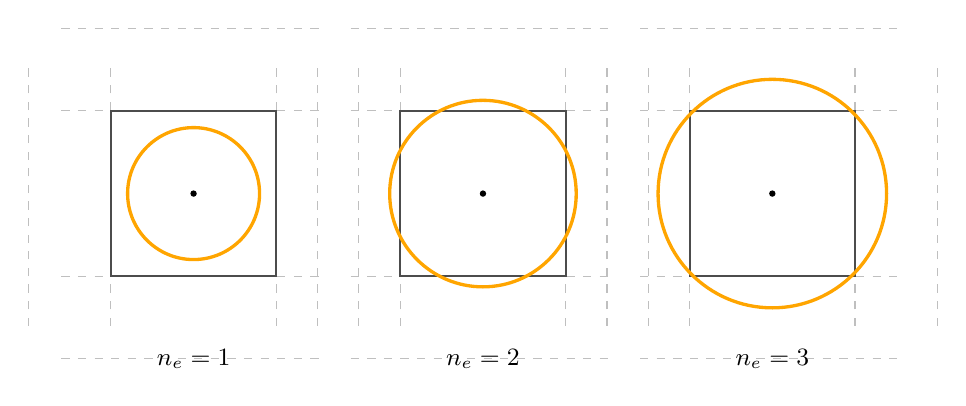
\begin{tikzpicture}[scale=1.05]
\foreach \n/\r/\xs in {1/0.798/0, 2/1.128/3.5, 3/1.382/7.0} {
  \begin{scope}[xshift=\xs cm]
    % extended zone boundaries
    \foreach \b in {-2,-1,1,2} {
      \draw[dashed, black!25] (\b,-1.6) -- (\b,1.6);
      \draw[dashed, black!25] (-1.6,\b) -- (1.6,\b);
    }
    % first Brillouin zone
    \draw[thick, black!70] (-1,-1) rectangle (1,1);
    % free-electron Fermi circle
    \draw[very thick, Orange] (0,0) circle (\r);
    \fill (0,0) circle (1.1pt);
    \node[font=\small] at (0,-2.0) {$n_e=\n$};
  \end{scope}
}
\end{tikzpicture}
\caption{The empty-lattice Fermi surface construction, shown for a two-dimensional square lattice where it can be drawn honestly in the plane. The free-electron circle of radius $k_F$ (orange) is superposed on the first Brillouin zone (solid) and the Bragg planes beyond it (dashed). For one electron per cell the circle fits inside the first zone; for two it has the zone's area but spills through the faces; for three it reaches into the second and third zones. The FCC case is the same construction with a sphere cut by the faces of the truncated octahedron.}
\label{fig:bloch-empty-fs}
\end{figure}

% ============================================================
\section{Band Sticking in Nonsymmorphic Crystals}
\label{sec:bloch-sticking}
% ============================================================

The degeneracies met so far have come from the geometry of the Bragg planes alone. A crystal's space group can force degeneracies of its own, and whether it does turns on the symmorphic--nonsymmorphic distinction of the previous chapter.

In a symmorphic crystal the symmetry operations that leave $\lvect{k}$ invariant --- the \emph{little group} of $\lvect{k}$ --- act on Bloch states as an ordinary point group, and the possible band degeneracies at that $\lvect{k}$ are read off from its irreducible representations. Nothing beyond the point group is involved.

In a nonsymmorphic crystal an operation carries an irremovable fractional translation $\lvect{\tau}$, and acting with it on a Bloch state produces an extra phase. If the operation returns a pure lattice translation after $n$ applications,
\begin{equation}
    \{R \mid \lvect{\tau}\}^n = \{E \mid \cvect{R}\}
    \quad\Longrightarrow\quad
    \bigl(\{R \mid \lvect{\tau}\}\bigr)^n \psi_{n\lvect{k}} = e^{-i\lvect{k}\cdot\cvect{R}}\,\psi_{n\lvect{k}} .
\end{equation}
Inside the zone this phase is harmless, but on the zone boundary it is nontrivial, and combined with the remaining symmetries it can force bands to be degenerate over entire lines or planes rather than at isolated points. This is called \emph{band sticking}.

The standard example is hcp, whose $6_3$ screw axis makes every band at least twofold degenerate across the whole hexagonal top face of the Brillouin zone, $k_z = \pi/c$. Degeneracies of this kind cannot occur in a symmorphic crystal, where no such phase is available; two bands that happen to meet there do so accidentally, and a small perturbation separates them.

% ============================================================
\section{The Tight-Binding Method}
% ============================================================

The weak-potential treatment above starts from plane waves and perturbs them with the ions. The opposite starting point is the isolated atom, which is appropriate whenever the solid is composed of weakly interacting neutral atoms.

\subsection{Assumptions}

We assume the solid is built from weakly interacting neutral atoms. Lower orbitals ($1s$, $2s$, $2p$, etc.) have less overlap between neighbouring atoms, so although the overlap is non-negligible we may still use single-atom atomic orbitals as a basis. The method is especially useful for describing $d$-shells of transition metals and for insulators.

\subsection{General Formulation}

Assume that in the vicinity of an atom the full Hamiltonian $H$ is well approximated by the single-atom Hamiltonian $H_{\text{at}}$,
\begin{equation}
    H_{\text{at}} \psi_n = E_n \psi_n,
\end{equation}
and require $\psi_n(\lvect{x})$ to be very small once $|\lvect{x}|$ exceeds the lattice constant $a$. Writing the crystal Hamiltonian as
\begin{equation}
    H = H_{\text{at}} + \Delta U(\lvect{x}),
\end{equation}
we have
\begin{equation}
    H \psi_n(\lvect{x}) = H_{\text{at}} \psi_n(\lvect{x}) + \Delta U(\lvect{x}) \psi_n(\lvect{x})
    = E_n \psi_n(\lvect{x}) + \boxed{\Delta U(\lvect{x})\psi_n(\lvect{x})}.
\end{equation}
For $\psi_n$ to satisfy the crystal Hamiltonian the boxed term must vanish, which happens either because $\Delta U(\lvect{x})$ is small (close to the atom) or because $\psi_n(\lvect{x})$ is small (far from the atom). Hence an atomic solution $\psi_n(\lvect{x} - \cvect{R})$ can be placed at each atomic site $\cvect{R}$ of the lattice.

These site-localized functions do not individually satisfy the Bloch condition $\psi(\lvect{x}+\cvect{R}) = e^{i\lvect{k}\cdot\cvect{R}}\psi(\lvect{x})$, so we take linear combinations,
\begin{equation}
    \psi_{n\lvect{k}}(\lvect{x}) = \sum_{\cvect{R}} e^{i\lvect{k}\cdot\cvect{R}}\, \psi_n(\lvect{x} - \cvect{R}),
    \label{eq:bloch-tb-sum}
\end{equation}
where $\lvect{k}$ lies in the first Brillouin zone with Born--von Karman boundary conditions.

\begin{theorem}[\eqref{eq:bloch-tb-sum} satisfies Bloch's theorem]
Let $\cvect{R}'' = \cvect{R}' - \cvect{R}$, which is again a lattice vector by the periodic boundary conditions. Then
\begin{align}
    \psi(\lvect{x}+\cvect{R}) &= \sum_{\cvect{R}'} e^{i\lvect{k}\cdot\cvect{R}'}\, \psi_n(\lvect{x} + \cvect{R} - \cvect{R}')
    = \sum_{\cvect{R}''} e^{i\lvect{k}\cdot(\cvect{R}''+\cvect{R})}\, \psi_n(\lvect{x} - \cvect{R}'') \\
    &= e^{i\lvect{k}\cdot\cvect{R}} \sum_{\cvect{R}''} e^{i\lvect{k}\cdot\cvect{R}''}\, \psi_n(\lvect{x} - \cvect{R}'')
    = e^{i\lvect{k}\cdot\cvect{R}}\, \psi(\lvect{x}).
\end{align}
\end{theorem}

However, acting with $H$ on this state,
\begin{equation}
    H\psi_{n\lvect{k}} = \sum_{\cvect{R}} e^{i\lvect{k}\cdot\cvect{R}} H \psi_n(\lvect{x}-\cvect{R}) = E_n \psi_{n\lvect{k}}(\lvect{x}),
\end{equation}
gives no modification to the atomic energies at all --- which is not realistic. The fix is to assume instead that the product $\Delta U(\lvect{x})\psi_n(\lvect{x})$ is exceedingly small but nonzero.

\begin{formula}[Tight-binding ansatz]
Assume a single-atom-like wavefunction $\phi(\lvect{x})$ close to the true $\psi(\lvect{x})$,
\begin{equation}
    \phi(\lvect{x}) = \sum_n b_n \psi_n(\lvect{x}) \qquad \text{(cf.\ Wannier functions)},
\end{equation}
and build the crystal state as
\begin{equation}
    \psi_{\lvect{k}}(\lvect{x}) = \sum_{\cvect{R}} e^{i\lvect{k}\cdot\cvect{R}}\, \phi(\lvect{x}-\cvect{R}),
    \qquad b_n = \braket{\psi_n | \phi}.
\end{equation}
\end{formula}

\subsection{Finding the Coefficients}

We need the $b_n(\lvect{k})$. Start from $H\ket{\psi_{\lvect{k}}} = (H_{\text{at}} + \Delta U)\ket{\psi_{\lvect{k}}} = \varepsilon(\lvect{k})\ket{\psi_{\lvect{k}}}$ and project onto an atomic orbital. Since $\bra{\psi_m} H_{\text{at}} \ket{\psi_{\lvect{k}}} = E_m \braket{\psi_m | \psi_{\lvect{k}}}$,
\begin{equation}
    \bra{\psi_m} H \ket{\psi_{\lvect{k}}} = E_m \braket{\psi_m|\psi_{\lvect{k}}} + \bra{\psi_m}\Delta U\ket{\psi_{\lvect{k}}} = \varepsilon(\lvect{k}) \braket{\psi_m|\psi_{\lvect{k}}},
\end{equation}
so that
\begin{equation}
    \bigl(\varepsilon(\lvect{k}) - E_m\bigr) \braket{\psi_m | \psi_{\lvect{k}}} = \bra{\psi_m} \Delta U \ket{\psi_{\lvect{k}}}.
\end{equation}
Now insert $\ket{\psi_{\lvect{k}}} = \sum_{\cvect{R}} e^{i\lvect{k}\cdot\cvect{R}} \sum_n b_n \ket{\psi_n(\lvect{x}-\cvect{R})}$ and use $\braket{\psi_m|\psi_n} = \delta_{mn}$:
\begin{equation}
    \bigl(\varepsilon(\lvect{k}) - E_m\bigr) \sum_n b_n \sum_{\cvect{R}} e^{i\lvect{k}\cdot\cvect{R}}
    \underbrace{\braket{\psi_m | \psi_n(\lvect{x}-\cvect{R})}}_{\displaystyle \alpha_{mn}(\cvect{R})}
    = \sum_n b_n \sum_{\cvect{R}} e^{i\lvect{k}\cdot\cvect{R}}
    \underbrace{\bra{\psi_m} \Delta U \ket{\psi_n(\lvect{x}-\cvect{R})}}_{\displaystyle \gamma_{mn}(\cvect{R})}.
\end{equation}
Rearranging gives the general constraint
\begin{equation}
    \varepsilon(\lvect{k}) \sum_n b_n \sum_{\cvect{R}} e^{i\lvect{k}\cdot\cvect{R}} \alpha_{mn}(\cvect{R})
    = \sum_n b_n \sum_{\cvect{R}} e^{i\lvect{k}\cdot\cvect{R}} \bigl( E_m \alpha_{mn}(\cvect{R}) + \gamma_{mn}(\cvect{R}) \bigr).
    \label{eq:bloch-tb-constraint}
\end{equation}

\subsection{The Tight-Binding Equation}

Assume now that $\alpha_{mn}(\cvect{R})$ and $\gamma_{mn}(\cvect{R})$ are negligible for $|\cvect{R}|$ beyond the nearest neighbours, so that the lattice sums run over a finite set. Define
\begin{equation}
    \alpha_{mn}(\lvect{k}) = \sum_{\text{n.n.}} e^{i\lvect{k}\cdot\cvect{R}} \alpha_{mn}(\cvect{R}),
    \qquad
    H_{mn}(\lvect{k}) = \sum_{\text{n.n.}} e^{i\lvect{k}\cdot\cvect{R}} H_{mn}(\cvect{R}),
    \qquad
    H_{mn}(\cvect{R}) = E_m \alpha_{mn}(\cvect{R}) + \gamma_{mn}(\cvect{R}).
\end{equation}
Then~\eqref{eq:bloch-tb-constraint} reads $\varepsilon(\lvect{k}) \sum_n b_n \alpha_{mn}(\lvect{k}) = \sum_n b_n H_{mn}(\lvect{k})$.

\begin{formula}[Tight-binding equation]
\begin{equation}
    \varepsilon(\lvect{k})\, \alpha(\lvect{k})\, \lvect{c} = H(\lvect{k})\, \lvect{c},
    \qquad \lvect{c} = (b_1, \ldots, b_n)^T.
\end{equation}
\end{formula}

\subsection{Application to an $s$-Band}

\begin{example}[Single $s$-band]
If there is only one band then $\alpha(\lvect{k}) = \mathbb{1}$ and $\lvect{c} \to 1$, so $\varepsilon(\lvect{k})\mathbb{1} = H(\lvect{k})$. With $\alpha_{mn}(\cvect{R}) = \delta_{mn}\delta_{\cvect{R},0}$,
\begin{equation}
    H(\lvect{k}) = \sum_{\text{n.n.}} e^{i\lvect{k}\cdot\cvect{R}} \bigl( E_m \delta_{\cvect{R},0} + \gamma(\cvect{R}) \bigr)
    = E_m - \beta + \sum_{\text{n.n.}} e^{i\lvect{k}\cdot\cvect{R}} \gamma(\cvect{R}),
\end{equation}
where $-\beta = \gamma(0)$ is the on-site term. By inversion symmetry of the lattice $\Delta U(-\cvect{R}) = \Delta U(\cvect{R})$, so $\gamma(\cvect{R}) = \gamma$ is the same for all nearest neighbours and the exponentials combine into cosines:
\begin{equation}
    \varepsilon(\lvect{k}) = E_s - \beta + \sum_{\text{n.n.}} \gamma \cos(\lvect{k}\cdot\cvect{R}).
\end{equation}
\end{example}

\begin{formula}[Single-orbital tight-binding]
\begin{equation}
    \varepsilon(\lvect{k}) = E_s - \beta - \sum_{\text{n.n.}} \gamma(\cvect{R}) \cos(\lvect{k}\cdot\cvect{R}),
    \qquad
    \gamma \equiv -\bra{\phi(\lvect{x})} \Delta U(\lvect{x}) \ket{\phi(\lvect{x}-\cvect{R})},
\end{equation}
where ``n.n.'' means only nearest-neighbour atomic separations are summed. The assumptions are:
\begin{enumerate}
    \item \emph{Orthogonality}: $\alpha(\cvect{R}) = \int d\lvect{x}\; \phi^*(\lvect{x})\phi(\lvect{x}-\cvect{R}) = 0$;
    \item only nearest-neighbour separations give appreciable overlap integrals.
\end{enumerate}
\end{formula}

\begin{example}[Tight-binding for an FCC crystal]
The 12 nearest neighbours of the origin in an FCC lattice sit at
\begin{equation}
    \cvect{R} = \tfrac{a}{2}(\pm 1, \pm 1, 0), \quad \tfrac{a}{2}(\pm 1, 0, \pm 1), \quad \tfrac{a}{2}(0, \pm 1, \pm 1),
\end{equation}
so $\lvect{k}\cdot\cvect{R} = \tfrac{a}{2}(\pm k_i \pm k_j)$ with $ij = xy,\, yz,\, xz$. Summing the twelve exponentials gives
\begin{equation}
    \varepsilon(\lvect{k}) = E_s - \beta - 4\gamma \sum_{ij} \cos(k_i a)\cos(k_j a).
\end{equation}
The intuition to carry away: the smaller the orbital overlap integral, the narrower the band.
\end{example}

\subsection{From Atomic Levels to Bands}

Figure~\ref{fig:bloch-levels} contrasts the discrete levels of an electron in a single-atom potential with what happens in a solid: as the atoms are brought together, each atomic level broadens into a band containing $N$ values of $\lvect{k}$.

\begin{figure}[ht]
\centering
\begin{tikzpicture}[scale=1.0]
    % --- left: single-atom potential with discrete levels ---
    \begin{scope}
        \draw[-{Stealth}] (0,0) -- (0,3.2) node[above] {$V(r)$};
        \draw[-{Stealth}] (-1.9,0) -- (2.4,0) node[right] {$r$};
        \draw[thick, domain=0.32:2.2, samples=100, variable=\t] plot ({\t}, {-0.9/\t + 1.4});
        \draw[thick, domain=-2.2:-0.32, samples=100, variable=\t] plot ({\t}, {0.9/\t + 1.4});
        \draw[dashed] (-1.9,0.35) -- (1.9,0.35) node[right, font=\small] {$n=1$};
        \draw[dashed] (-1.5,0.95) -- (1.5,0.95) node[right, font=\small] {$n=2$};
        \draw[dashed] (-1.2,1.3) -- (1.2,1.3) node[right, font=\small] {$n=3$};
        \node[align=center, font=\small] at (0.2,-0.75) {electronic levels in\\a single-atom potential};
    \end{scope}
    % --- right: levels broadening into bands ---
    \begin{scope}[xshift=6.6cm]
        \draw[-{Stealth}] (0,0) -- (0,3.2) node[above, font=\small] {energy levels};
        \draw[-{Stealth}] (0,3.0) -- (2.6,3.0) node[right, font=\small] {spacing};
        \draw (0,0.35) -- (2.2,0.05);
        \draw (0,0.35) -- (2.2,0.65);
        \draw (0,1.25) -- (2.2,0.85);
        \draw (0,1.25) -- (2.2,1.65);
        \draw (0,1.95) -- (2.2,1.5);
        \draw (0,1.95) -- (2.2,2.4);
        \draw[decorate, decoration={brace, amplitude=5pt}] (2.5,2.45) -- (2.5,0.0);
        \node[right, align=left, font=\small] at (2.75,1.2) {bands, each with\\$N$ values of $\lvect{k}$};
        \node[align=center, font=\small] at (1.1,-0.75) {electronic levels\\in a solid};
    \end{scope}
\end{tikzpicture}
\caption{Discrete levels of the single-atom potential (left) broaden into bands as the atomic spacing is reduced (right); each band contains $N$ allowed values of $\lvect{k}$.}
\label{fig:bloch-levels}
\end{figure}

\subsection{Remarks on the Tight-Binding Method}

\begin{enumerate}
    \item The number of atomic levels kept in the expansion determines the number of bands, and equals the dimension of the matrix problem --- as one sees from the indices of $H_{mn}$.
    \item The width of a band (lowest to highest energy within it) scales with the overlap integrals $\gamma_{mn}(\cvect{R})$. Rule of thumb: as the energy of a given atomic level increases, so does the spatial extent of its wavefunction.
    \item The more overlap, the greater $\partial\varepsilon/\partial \lvect{k}$, which means the electrons have a larger mean velocity.
    \item For materials with more than one atom in the basis, use
    \begin{equation}
        \psi(\lvect{x}) = \sum_{\cvect{R}} e^{i\lvect{k}\cdot\cvect{R}}\bigl( a\,\phi(\lvect{x}-\cvect{R}) + b\,\phi(\lvect{x}-\lvect{d}-\cvect{R}) \bigr).
    \end{equation}
    \item When spin--orbit coupling is present (as in heavier elements), include in $\Delta U(\lvect{x})$ the electron's interaction with neighbouring atomic spins, and approximate $\phi$ as a linear combination of the same orbital wavefunctions but of opposite spin --- which doubles the size of the tight-binding matrix.
    \item The method still assumes the independent-electron approximation, and so fails for magnetic materials.
\end{enumerate}

\subsection{Wannier Functions}

Wannier functions form a basis for the atomic wavefunctions $\phi$. Any Bloch function can be written in the form
\begin{equation}
    \psi_{n\lvect{k}}(\lvect{x}) = \sum_{\cvect{R}} e^{i\lvect{k}\cdot\cvect{R}} f_n(\cvect{R}, \lvect{x}),
    \qquad
    f_n(\cvect{R},\lvect{x}) = \frac{1}{v_0} \int d\lvect{k}\; e^{-i\lvect{k}\cdot\cvect{R}} \psi_{n\lvect{k}}(\lvect{x}),
\end{equation}
and by Bloch's theorem it must be that $f_n(\cvect{R},\lvect{x}) = \phi_n(\lvect{x}-\cvect{R})$.

\begin{fact}[Orthogonality]
\begin{equation}
    \braket{\phi_n | \phi_m} = \braket{\phi_n(\lvect{x}-\cvect{R}_a) | \phi_n(\lvect{x}-\cvect{R}_b)} = 0.
\end{equation}
\end{fact}

Because they are localized, Wannier functions are important for modelling semiclassical electron transport and defect states in semiconductors.

% ============================================================
\section{Lattice Fourier Transforms and Identities}
% ============================================================

Both models above lean on a handful of lattice Fourier identities, which we now collect. The starting point is that the plane waves $e^{i\lvect{k}\cdot\lvect{x}}$ form a complete basis for any well-behaved function on $\mathbb{R}^3$.

\subsection{Functions Periodic in Real Space}

If $f(\lvect{x}+\cvect{R}) = f(\lvect{x})$, then only those plane waves periodic in the lattice can appear --- that is, those with reciprocal lattice wavevectors:
\begin{equation}
    f(\lvect{x}) = \sum_{\cvect{G}} f_{\cvect{G}}\, e^{i\cvect{G}\cdot\lvect{x}},
    \qquad
    f_{\cvect{G}} = \frac{1}{v}\int_C d\lvect{x}\; e^{-i\cvect{G}\cdot\lvect{x}} f(\lvect{x}),
\end{equation}
where the integral runs over any primitive cell $C$ of volume $v$.

\begin{theorem}[Vanishing of the cell integral]
For a nonzero reciprocal lattice vector $\cvect{G}$, $\int_C d\lvect{x}\, e^{i\cvect{G}\cdot\lvect{x}} = 0$. Translating the unit cell does not change the integral, so
\begin{equation}
    \int_C d\lvect{x}\; e^{i\cvect{G}\cdot\lvect{x}} = \int_C d\lvect{x}\; e^{i\cvect{G}\cdot(\lvect{x}+\lvect{d})}
    \;\Longrightarrow\;
    \left(\int_C d\lvect{x}\; e^{i\cvect{G}\cdot\lvect{x}}\right)\bigl(e^{i\cvect{G}\cdot\lvect{d}} - 1\bigr) = 0.
\end{equation}
The second factor is never zero for generic $\lvect{d}$, so the integral vanishes.
\end{theorem}

\subsection{Functions Periodic in Reciprocal Space}

Dually, a function periodic in reciprocal space is expanded on direct lattice vectors:
\begin{equation}
    \phi(\lvect{k}) = \sum_{\cvect{R}} e^{i\cvect{R}\cdot\lvect{k}}\, \phi_{\cvect{R}},
    \qquad
    \phi_{\cvect{R}} \equiv V \int \frac{d\lvect{k}}{(2\pi)^3}\, e^{-i\cvect{R}\cdot\lvect{k}}\, \phi(\lvect{k}).
\end{equation}

\subsection{Functions Periodic under Born--von Karman Boundary Conditions}

The BVK boundary condition is $f(\lvect{x} + N_i \lvect{a}_i) = f(\lvect{x})$, which restricts the allowed wavevectors to
\begin{equation}
    \lvect{k} = \sum_{i=1}^{3} \frac{m_i}{N_i}\, \lvect{b}_i, \qquad m_i \in \mathbb{Z}.
\end{equation}
The expansion then takes the form
\begin{equation}
    f(\lvect{x}) = \sum_{\lvect{k}} f_{\lvect{k}}\, e^{i\lvect{k}\cdot\lvect{x}},
    \qquad
    f_{\lvect{k}} \equiv \frac{1}{V}\int d\lvect{x}\; e^{-i\lvect{k}\cdot\lvect{x}} f(\lvect{x}),
\end{equation}
and again $\int_V d\lvect{x}\, e^{i\lvect{k}\cdot\lvect{x}} = 0$ for $\lvect{k} \neq 0$.

\begin{theorem}[Sum of exponentials identity]
For $\cvect{R}$ running over the lattice sites $\sum_{i=1}^3 n_i \lvect{a}_i$ with $0 \leq n_i < N_i$ and $N_1 N_2 N_3 = N$,
\begin{equation}
    \sum_{\cvect{R}} e^{i\lvect{k}\cdot\cvect{R}} = N \delta_{\lvect{k},0}.
\end{equation}
The sum is invariant under displacing every site by a lattice vector $\cvect{R}_0$,
\begin{equation}
    \sum_{\cvect{R}} e^{i\lvect{k}\cdot(\cvect{R}+\cvect{R}_0)} = e^{i\lvect{k}\cdot\cvect{R}_0} \sum_{\cvect{R}} e^{i\lvect{k}\cdot\cvect{R}} = \sum_{\cvect{R}} e^{i\lvect{k}\cdot\cvect{R}},
\end{equation}
so that $\bigl(e^{i\lvect{k}\cdot\cvect{R}_0} - 1\bigr)\bigl(\sum_{\cvect{R}} e^{i\lvect{k}\cdot\cvect{R}}\bigr) = 0$. If $\lvect{k} = 0$ the sum is $\sum_{\cvect{R}} 1 = N$; if $\lvect{k} \neq 0$ the sum must vanish.
\end{theorem}

\begin{formula}[BVK identity]
\begin{equation}
    \sum_{\lvect{k}} e^{i\lvect{k}\cdot\cvect{R}} = N \delta_{\cvect{R},0}.
\end{equation}
\end{formula}

% ============================================================
\section{Wave Packets of Bloch Electrons}
% ============================================================

In the semiclassical picture electrons do \emph{not} collide with the ions --- the mean free path is far too long for that --- but rather with imperfections in the crystal. To describe their response to applied fields we build wavepackets out of Bloch states.

\begin{definition}[Bloch wavepacket]
\begin{equation}
    \psi_n(\lvect{x},t) = \sum_{\lvect{k}'} g(\lvect{k}')\, \psi_{n\lvect{k}'}(\lvect{x})\, \exp\!\left(-\tfrac{i}{\hbar}\varepsilon_n(\lvect{k}')t\right),
\end{equation}
where the weight $g(\lvect{k}') \approx 0$ once $|\lvect{k}'-\lvect{k}| > \Delta k$. The packet must obey the uncertainty principle $\Delta k\, \Delta x \gtrsim 1$.
\end{definition}

\subsection{Width of the Wavepacket}

Assume $\Delta k$ is small compared with the dimensions of the Brillouin zone, and examine the amplitude at points a lattice vector away:
\begin{equation}
    \psi_n(\lvect{x}_0 + \cvect{R}, t) = \sum_{\lvect{k}'} \underbrace{\bigl[ g(\lvect{k}')\psi_{n\lvect{k}'}(\lvect{x}_0) \bigr]}_{\text{weight function}}
    \exp\!\left[ i\Bigl( \underbrace{\lvect{k}'\cdot\cvect{R}}_{\text{from the Bloch condition}} - \tfrac{1}{\hbar}\varepsilon_n(\lvect{k}')t \Bigr) \right].
\end{equation}
By the properties of the Fourier transform, if $g(\lvect{k})$ is appreciable within $\Delta k$ then $g(\lvect{x})$ is appreciable within $\Delta R \approx 1/\Delta k$. Since $\Delta k$ is small compared with the Brillouin zone dimension, of order $1/a$, the spread $\Delta R$ is large compared with the lattice constant $a$: wavepackets are spread over many primitive unit cells.

\subsection{Group Velocity of Bloch Electrons}

Expand the band energy to second order in a small shift $\lvect{q}$:
\begin{equation}
    \varepsilon_n(\lvect{k}+\lvect{q}) = \varepsilon_n(\lvect{k}) + \sum_i \pdv{\varepsilon_n}{k_i} q_i
    + \frac{1}{2}\sum_{ij} \frac{\partial^2 \varepsilon_n}{\partial k_i \partial k_j} q_i q_j + O(q^3).
    \label{eq:bloch-expand}
\end{equation}
The same shift can be treated by perturbation theory: since $H_{\lvect{k}+\lvect{q}}\psi^n_{\lvect{k}+\lvect{q}} = \varepsilon^n_{\lvect{k}+\lvect{q}}\psi^n_{\lvect{k}+\lvect{q}}$,
\begin{equation}
    H_{\lvect{k}+\lvect{q}} = H_{\lvect{k}} + \underbrace{\frac{\hbar^2}{m}\,\lvect{q}\cdot\left(\frac{1}{i}\nabla + \lvect{k}\right)}_{\displaystyle V(\lvect{q})} + \frac{\hbar^2}{2m}q^2 .
    \label{eq:bloch-Hexpand}
\end{equation}
If the unperturbed problem is $H_0 \psi_n = E^0_n \psi_n$, then to second order in $V$,
\begin{equation}
    E_n = E^0_n + \int d\lvect{x}\; \psi_n^* V \psi_n + \sum_{n' \neq n} \frac{\bigl| \int d\lvect{x}\; \psi_n^* V \psi_{n'} \bigr|^2}{E^0_n - E^0_{n'}}.
    \label{eq:bloch-pert}
\end{equation}
Comparing~\eqref{eq:bloch-expand} with~\eqref{eq:bloch-pert} at first order,
\begin{equation}
    \sum_i \pdv{\varepsilon_n}{k_i} q_i = \int d\lvect{x}\; \psi_n^* V \psi_n,
\end{equation}
and comparing~\eqref{eq:bloch-Hexpand} with~\eqref{eq:bloch-pert} we need the part of $V(\lvect{q})$ linear in $\lvect{q}$, so that
\begin{equation}
    \sum_i \pdv{\varepsilon_n}{k_i} q_i = \frac{\hbar^2}{m} \sum_i \int d\lvect{x}\; u^*_{n\lvect{k}}\, q_i \left(\frac{1}{i}\nabla + \lvect{k}\right)_{\!i} u_{n\lvect{k}}.
\end{equation}
Recalling the momentum operator $\hat{p}_i \equiv \frac{\hbar}{i}\pdv{}{x_i}$,
\begin{equation}
    \frac{1}{\hbar}\pdv{\varepsilon_n}{k_i} = \frac{1}{m} \Bigl\langle \frac{\hbar}{i}\pdv{}{x_i} + \hbar k_i \Bigr\rangle_{u_{n\lvect{k}}}
    = \frac{1}{m}\bigl\langle \hat{p}_i + \hbar k_i \bigr\rangle_{u_{n\lvect{k}}}.
\end{equation}
Finally, using $\psi_{n\lvect{k}} = e^{i\lvect{k}\cdot\lvect{x}} u_{n\lvect{k}}(\lvect{x})$,
\begin{equation}
    \frac{1}{\hbar}\pdv{\varepsilon_n}{k_i}
    = \frac{1}{m}\int d\lvect{x}\; u^*_{n\lvect{k}} (\hat{p}_i + \hbar k_i) u_{n\lvect{k}}
    = \frac{1}{m}\int d\lvect{x}\; e^{i\lvect{k}\cdot\lvect{x}} \psi^*_{n\lvect{k}} (\hat{p}_i + \hbar k_i) e^{-i\lvect{k}\cdot\lvect{x}} \psi_{n\lvect{k}},
\end{equation}
and since
\begin{equation}
    \hat{p}_i \bigl[ e^{-i\lvect{k}\cdot\lvect{x}} \psi_{n\lvect{k}}(\lvect{x}) \bigr]
    = \frac{\hbar}{i}\pdv{}{x_i}\bigl[ e^{-i\lvect{k}\cdot\lvect{x}} \psi_{n\lvect{k}}(\lvect{x}) \bigr]
    = -\hbar k_i\, e^{-i\lvect{k}\cdot\lvect{x}}\psi_{n\lvect{k}}(\lvect{x}) + e^{-i\lvect{k}\cdot\lvect{x}}\, \hat{p}_i \psi_{n\lvect{k}}(\lvect{x}),
\end{equation}
the $\hbar k_i$ terms cancel, leaving
\begin{equation}
    \frac{1}{\hbar}\pdv{\varepsilon_n}{k_i}
    = \frac{1}{m}\int d\lvect{x}\; e^{i\lvect{k}\cdot\lvect{x}} \psi^*_{n\lvect{k}} e^{-i\lvect{k}\cdot\lvect{x}} \hat{p}_i \psi_{n\lvect{k}}
    = \frac{1}{m}\langle \hat{p}_i \rangle_{\psi_{n\lvect{k}}} = \langle \hat{v}_i \rangle_{\psi_{n\lvect{k}}}.
\end{equation}

\begin{formula}[Group velocity]
\begin{equation}
    \langle \lvect{v}_n(\lvect{k}) \rangle = \frac{1}{\hbar} \pdv{\varepsilon_n(\lvect{k})}{\lvect{k}} = \pdv{\omega}{\lvect{k}}.
\end{equation}
\end{formula}

% ============================================================
\section{The Semiclassical Model}
% ============================================================

The semiclassical model describes the response of electrons to externally applied electric and magnetic fields that vary slowly on the scale $\Delta R$ of the wavepacket. Given the band structure $\varepsilon_n(\lvect{k})$, it associates with each electron a position $\lvect{x}$, a wavevector $\lvect{k}$, and a band index $n$.

\begin{fact}[Assumptions of the semiclassical model]
\begin{enumerate}
    \item The electron stays within its band: there are no interband transitions.
    \item The time evolution is governed by
    \begin{equation}
        \dot{\lvect{x}} = \lvect{v}_n(\lvect{k}) = \frac{1}{\hbar}\pdv{\varepsilon_n(\lvect{k})}{\lvect{k}},
        \qquad
        \hbar \dot{\lvect{k}} = -e\left[ \cvect{E}(\lvect{x},t) + \frac{1}{c}\, \lvect{v}_n(\lvect{k}) \times \cvect{H}(\lvect{x},t) \right],
    \end{equation}
    where $\cvect{H}$ is the magnetic field. Note that the crystal momentum $\hbar\lvect{k}$ is \emph{not} the total electron momentum.
    \item All distinct wavevectors for a single band lie within a single primitive cell of the reciprocal lattice, with occupation given by the Fermi distribution
    \begin{equation}
        f\bigl(\varepsilon_n(\lvect{k})\bigr) \frac{d\lvect{k}}{4\pi^3}
        = \frac{d\lvect{k}/4\pi^3}{e^{(\varepsilon_n(\lvect{k})-\mu)/k_B T}+1}.
    \end{equation}
\end{enumerate}
\end{fact}

A useful corollary is the \emph{many-carrier} statement: one need only consider the types of carriers lying within $\sim k_B T$ of the Fermi level.

\subsection{Conditions of Validity}

There must be some minimum strength of the periodic potential below which the model breaks down, because interband transitions become possible. The conditions are
\begin{equation}
    e |\cvect{E}| a \ll \frac{\bigl[\varepsilon_{\text{gap}}(\lvect{k})\bigr]^2}{\varepsilon_F},
    \qquad
    \hbar\omega_c \ll \frac{\bigl[\varepsilon_{\text{gap}}(\lvect{k})\bigr]^2}{\varepsilon_F},
\end{equation}
where $\omega_c$ is the cyclotron frequency: both the work done by the field over a lattice constant and the cyclotron energy quantum must be small compared with the scale set by the gap.

\subsection{Bloch Oscillations}

Apply the model to an electron in a single band of a one-dimensional crystal of lattice constant $a$, in a uniform static field $E$ and no magnetic field. The Hamiltonian is
\begin{equation}
    H = \frac{p^2}{2m} + U(x) + eEx,
\end{equation}
and the equation of motion reduces to
\begin{equation}
    \hbar\dot{k} = -eE \qquad\Longrightarrow\qquad k(t) = k(0) - \frac{eEt}{\hbar}.
\end{equation}
The wavevector therefore moves uniformly through the Brillouin zone. On reaching one zone boundary it re-enters from the opposite one, since $k = \pm\pi/a$ label the same state: the one-dimensional Brillouin zone is topologically a circle. The velocity $v_n(k) = \hbar^{-1}\,\partial\varepsilon_n/\partial k$ is periodic in $k$ and changes sign across the zone, so the electron does not accelerate indefinitely but oscillates.

\begin{formula}[Bloch oscillation period]
\begin{equation}
    T_B = \frac{2\pi\hbar}{eEa}, \qquad \nu_B = \frac{eEa}{h}.
\end{equation}
\end{formula}

Integrating the velocity shows the real-space motion is bounded as well. For a tight-binding $s$-band $\varepsilon(k) = -2\gamma\cos ka$,
\begin{equation}
    x(t)-x(0) = \frac{1}{\hbar}\int_0^t \pdv{\varepsilon}{k}\,dt'
    = \frac{\varepsilon\bigl(k(t)\bigr) - \varepsilon\bigl(k(0)\bigr)}{-eE},
\end{equation}
so the amplitude of the oscillation is the bandwidth divided by the force, $4\gamma/eE$.

\begin{fact}[Consequences of Bloch oscillations]
\begin{enumerate}
    \item A \emph{static} electric field produces an \emph{oscillating} current: a perfect crystal would act as a DC-to-AC converter.
    \item In real solids the oscillations are almost never seen, because the scattering time from impurities and phonons is much shorter than $T_B$. They have been observed directly with cold atoms in optical lattices, and in semiconductor superlattices, where the large period $a$ shortens $T_B$.
    \item At strong fields the electron can tunnel into a higher band instead of Bragg reflecting. This \emph{Zener tunnelling} is exactly the interband transition excluded by the validity condition on $e|\cvect{E}|a$ above.
\end{enumerate}
\end{fact}
